\documentclass[
  a4paper,
  oneside,
  BCOR = 10mm,
  DIV = 12,
  12pt,
  headings = normal,
]{scrartcl}

%%% Length calculations
\usepackage{calc}
%%%

%%% Support for color
\usepackage{xcolor}
\definecolor{lightblue}{HTML}{03A9F4}
\definecolor{red}{HTML}{F44336}
%%%

%%% Including graphics
\usepackage{graphicx}
%%%

%%% Font selection
\usepackage{fontspec}

\setromanfont{STIX Two Text}[
  SmallCapsFeatures = {LetterSpace = 8},
]

\setsansfont{IBM Plex Sans}[
  Scale = MatchUppercase,
]

\setmonofont{IBM Plex Mono}[
  Scale = MatchUppercase,
]
%%%

%%% Math typesetting
\usepackage{amsmath}

\usepackage{unicode-math}
\setmathfont{STIX Two Math}

\usepackage{IEEEtrantools}
%%%

%%% List settings
\usepackage{enumitem}
\setlist[enumerate]{
  label*      = {\arabic*.},
  left        = \parindent,
  topsep      = 0\baselineskip,
  parsep      = 0\baselineskip,
  noitemsep, % override itemsep
}
% List settings for levels 2–4
\setlist[enumerate, 2, 3, 4]{
  label*      = {\arabic*.},
  left        = 0em,
  topsep      = 0\baselineskip,
  parsep      = 0\baselineskip,
  noitemsep, % override itemsep
}

\setlist[itemize]{
  label*      = {—},
  left        = \parindent,
  topsep      = 0\baselineskip,
  parsep      = 0\baselineskip,
  itemsep     = 1\baselineskip,
  noitemsep, % override itemsep
}

\setlist[description]{
  font        = {\rmfamily\upshape\bfseries},
  topsep      = 1\baselineskip,
  parsep      = 0\baselineskip,
  itemsep     = 0\baselineskip,
}

%%%

%%% Structural elements typesetting
\setkomafont{pagenumber}{\rmfamily\upshape}
\setkomafont{disposition}{\rmfamily\bfseries}

% Sectioning
\RedeclareSectionCommand[
  beforeskip = -1\baselineskip,
  afterskip  = 1\baselineskip,
  font       = {\normalsize\bfseries\scshape},
]{section}

\RedeclareSectionCommand[
  beforeskip = -1\baselineskip,
  afterskip  = 1\baselineskip,
  font       = {\normalsize\bfseries\itshape},
]{subsection}

\RedeclareSectionCommand[
  beforeskip = -1\baselineskip,
  afterskip  = 1\baselineskip,
  font       = {\normalsize\bfseries},
]{subsubsection}

\RedeclareSectionCommand[
  beforeskip = -1\baselineskip,
  afterskip  = -0.5em,
  font       = {\normalsize\mdseries\scshape\addfontfeatures{Letters = {UppercaseSmallCaps}}},
]{paragraph}
%%%

%%% Typographic enhancements
\usepackage{microtype}
%%%

%%% Language-specific settings
\usepackage{polyglossia}
\setmainlanguage{ukrainian}
\setotherlanguages{english}
%%%

%%% Captions
\usepackage{caption}
\usepackage{subcaption}

%\DeclareCaptionLabelFormat{closing}{#2)}
%\captionsetup[subtable]{labelformat = closing}

%\captionsetup[subfigure]{labelformat = closing}

\captionsetup[table]{
  aboveskip = 0\baselineskip,
  belowskip = 0\baselineskip,
}

\captionsetup[figure]{
  aboveskip = 1\baselineskip,
  belowskip = 0\baselineskip,
}

\captionsetup[subfigure]{
  labelformat = simple,
  labelformat = brace,
  justification = RaggedRight,
  singlelinecheck = false,
}
%%%

%%% Hyphenated ragged typesetting
\usepackage{ragged2e}
%%%

%%% Table typesetting
\usepackage{booktabs}
\usepackage{longtable}

\usepackage{multirow}

\usepackage{array}
\newcolumntype{v}[1]{>{\RaggedRight\arraybackslash\hspace{0pt}}p{#1}}
\newcolumntype{b}[1]{>{\Centering\arraybackslash\hspace{0pt}}p{#1}}
\newcolumntype{n}[1]{>{\RaggedLeft\arraybackslash\hspace{0pt}}p{#1}}
%%%

%%% Drawing
\usepackage{tikz}
\usepackage{tikzscale}
\usetikzlibrary{datavisualization}
\usetikzlibrary{datavisualization.formats.functions}
\usetikzlibrary{positioning}
\usetikzlibrary{patterns}
\usetikzlibrary{intersections}
\usetikzlibrary{arrows.meta} % Stealth arrow tips

\usepackage{pgfplots}
\usepgfplotslibrary{fillbetween}
%%%

%%% SI units typesetting
\usepackage{siunitx}
\sisetup{
  output-decimal-marker = {,},
  exponent-product      = {\cdot},
  inter-unit-product    = \ensuremath{{} \cdot {}},
  per-mode              = symbol,
}
%%%

% Code Highlighting
\usepackage{minted}
\setmintedinline{
  style = bw,
  breaklines,
}

\newminted[bashterm]{text}{%
  autogobble,%
  breaklines,%
  style=bw,%
}

\newminted[codegeneric]{text}{%
  autogobble,%
  style=bw,%
  breaklines,%
  fontsize=\small,%
}

\newmintinline{bash}{%
}

\newmintinline[minttext]{text}{%
  breaklines,%
  breakanywhere,%
}

%%% Framing code listings
\usepackage{tcolorbox}
\tcbuselibrary{breakable}
\tcbuselibrary{minted}
\tcbuselibrary{skins}

% Text file listing
\newtcblisting[
  auto counter,
  list inside,
  number within = section,
]{listingplaintext}[3][]{%
  minted language = text,
  minted style    = bw,
  minted options  = {
    autogobble,
    linenos,
    tabsize = 4,
    breaklines,
    breakanywhere,
    fontsize = \footnotesize,
  },
  empty,
  sharp corners,
  coltitle = black,
  borderline horizontal = {1pt}{0pt}{black},
  titlerule = {0.5pt},
  titlerule style = {
    black,
  },
  toptitle = 0.3em,
  bottomtitle = 0.3em,
  before skip      = \intextsep,
  after  skip      = \intextsep,
  title            = {Лістинг \thetcbcounter: #2},
  list entry       = {\protect\numberline{\thetcbcounter}#2},
  left = 0em,
  right = 0em,
  %
  listing only,
  breakable,
  %
  label = {#3},%
}

\newtcblisting[
  use counter from = listingplaintext,
  list inside,
  number within = section,
]{listingpython}[3][]{%
  minted language = python,
  minted style    = bw,
  minted options  = {
    autogobble,
    linenos,
    tabsize = 4,
    breaklines,
    breakanywhere,
    fontsize = \footnotesize,
  },
  empty,
  sharp corners,
  coltitle = black,
  borderline horizontal = {1pt}{0pt}{black},
  titlerule = {0.5pt},
  titlerule style = {
    black,
  },
  toptitle = 0.3em,
  bottomtitle = 0.3em,
  before skip      = \intextsep,
  after  skip      = \intextsep,
  title            = {Лістинг \thetcbcounter: #2},
  list entry       = {\protect\numberline{\thetcbcounter}#2},
  left = 0em,
  right = 0em,
  %
  listing only,
  breakable,
  %
  label = {#3},
  %
  #1%
}

\newtcbinputlisting[
  use counter from = listingplaintext,
  list inside,
  number within = section
]{\inputpython}[4][]{%
  minted language = python,
  minted style    = bw,
  minted options  = {
    autogobble,
    linenos,
    tabsize = 4,
    breaklines,
    breakanywhere,
    fontsize = \footnotesize,
  },
  empty,
  sharp corners,
  coltitle = black,
  borderline horizontal = {1pt}{0pt}{black},
  titlerule = {0.5pt},
  titlerule style = {
    black,
  },
  toptitle = 0.3em,
  bottomtitle = 0.3em,
  before skip      = \intextsep,
  after  skip      = \intextsep,
  title            = {Лістинг \thetcbcounter: #3},
  list entry       = {\protect\numberline{\thetcbcounter}#3},
  left = 0em,
  right = 0em,
  %
  listing file={#2},
  listing only,
  breakable,
  %
  label = {#4}
}

% Linux command-line listing
\newtcblisting{linuxterm}%
{%
  % Syntax highlighing options
  listing only,%
  minted language = bash,%
  minted options={%
    autogobble,%
    linenos%
  },%
  % Presentation options
  empty,%
  %% Margins
  sharp corners,%
  toptitle = 0.0em,%
  bottomtitle = 0.0em,%
  left = 0em,%
  right = 0em,%
  before skip = \intextsep,%
  after skip = \intextsep,%
}

\newtcblisting{linuxtermout}%
{%
  % Syntax highlighing options
  listing only,%
  minted language = text,%
  minted options={%
    autogobble,%
    linenos%
  },%
  % Presentation options
  empty,%
  %% Margins
  sharp corners,%
  toptitle = 0.0em,%
  bottomtitle = 0.0em,%
  left = 0em,%
  right = 0em,%
  before skip = \intextsep,%
  after skip = \intextsep,%
}

% Dockerfile listings
\newtcblisting[
  use counter from = listingplaintext,
  list inside,
  number within = section,
]{listingdocker}[3][]{%
  minted language = dockerfile,
  minted style    = bw,
  minted options  = {
    autogobble,%
    linenos,
    tabsize = 4,
    breaklines,
    breakanywhere,
    fontsize = \footnotesize,
  },
  empty,
  sharp corners,
  coltitle = black,
  borderline horizontal = {1pt}{0pt}{black},
  titlerule = {0.5pt},
  titlerule style = {
    black,
  },
  toptitle = 0.3em,
  bottomtitle = 0.3em,
  before skip      = \intextsep,
  after  skip      = \intextsep,
  title            = {Лістинг \thetcbcounter: #2},
  list entry       = {\protect\numberline{\thetcbcounter}#2},
  left = 0em,
  right = 0em,
  %
  listing only,
  breakable,
  %
  label = {#3},%
}

% Docker Compose listings
\newtcblisting[
  use counter from = listingplaintext,
  list inside,
  number within = section,
]{listingdockercompose}[3][]{%
  minted language = yaml,
  minted style    = bw,
  minted options  = {
    autogobble,%
    linenos,
    tabsize = 4,
    breaklines,
    breakanywhere,
    fontsize = \footnotesize,
  },
  empty,
  sharp corners,
  coltitle = black,
  borderline horizontal = {1pt}{0pt}{black},
  titlerule = {0.5pt},
  titlerule style = {
    black,
  },
  toptitle = 0.3em,
  bottomtitle = 0.3em,
  before skip      = \intextsep,
  after  skip      = \intextsep,
  title            = {Лістинг \thetcbcounter: #2},
  list entry       = {\protect\numberline{\thetcbcounter}#2},
  left = 0em,
  right = 0em,
  %
  listing only,
  breakable,
  %
  label = {#3},%
}


% Customize minted line numbers
\renewcommand{\theFancyVerbLine}{\ttfamily\scriptsize\arabic{FancyVerbLine}}

%%%

%%% Typeset menus and keys
\usepackage{menukeys}[
  os=win,
]
%%%

%%% Links and hyperreferences
\usepackage{hyperref}
\hypersetup{
  bookmarksnumbered = true,
  colorlinks      = false,
  linkbordercolor = red,
  urlbordercolor  = lightblue,
  pdfborderstyle  = {/S/U/W 1.5},
}
%%%

%%% Length adjustment

% Set baselineskip, default is 14.5 pt
\linespread{1.068966} % ~15.5 pt
\setlength{\emergencystretch}{1em}
\setlength{\parindent}{1.5em}
\newlength{\gridunitwidth}
\setlength{\gridunitwidth}{\textwidth / 12}
%%%

%%% Custom commands
\newcommand{\allcaps}[1]{%
  {%
    \addfontfeatures{%
      Letters = UppercaseSmallCaps,
      LetterSpace = 8,%
    }%
    #1%
  }%
}
\newcommand{\filename}[1]{\texttt{#1}}
\newcommand{\progname}[1]{\texttt{#1}}
\newcommand{\commandname}[1]{\texttt{#1}}
\newcommand{\modulename}[1]{\texttt{#1}}
\newcommand{\transeng}[1]{{англ.}~\textit{\textenglish{#1}}}
%%%

%%% Custom math commands
\newcommand{\longvar}[1]{\mathit{#1}}
%%%

\begin{document}

\begin{titlepage}
    \begin{center}
      Міністерство освіти і~науки України\\
      Національний авіаційний університет\\
      Факультет кібербезпеки, комп'ютерної та~програмної інженерії\\
      Кафедра комп'ютеризованих систем управління

      \vspace{\fill}
        Лабораторна робота №~1.2\\
        з~дисципліни «Дослідження операцій»\\
        на~тему «Побудова оптимізаційних економіко-математичних моделей. Графічний метод розв'язку задачі лінійного програмування»

      \vspace{\fill}

      \begin{flushright}
        Виконав:\\
        студент \allcaps{ФККПІ}\\
        групи \allcaps{СП}-425\\
        Клокун В.\,Д.\\
        Перевірила:\\
        Яковенко Л.\,В.
      \end{flushright}

      Київ 2019
    \end{center}
  \end{titlepage}

  \section{Завдання роботи}
    Розв'язати графічним методом:
    \begin{IEEEeqnarray*}{c}
      L = -4 x_{1} - 5 x_{2} \to \min,\\
      \left\{ \,
        \begin{IEEEeqnarraybox}[
          \IEEEeqnarraystrutmode
          \IEEEeqnarraystrutsizeadd{2pt}{2pt}
        ][c]{rCrCl}
          4 x_{1} &+&  5 x_{2} &\leqslant& 20, \\
          - x_{1} &+& 10 x_{2} &\geqslant& 10, \\
          7 x_{1} &+&  5 x_{2} &\leqslant& 35, \\
            x_{1} & \leqslant& \multicolumn{1}{l}{7,} \\
            x_{2} & \leqslant& \multicolumn{1}{l}{4,} \\
            x_{1} & \geqslant& \multicolumn{1}{l}{0,} \\
            x_{2} & \geqslant& \multicolumn{1}{l}{0.}
        \end{IEEEeqnarraybox}
      \right.
    \end{IEEEeqnarray*}

  \section{Хід~роботи}
    Щоб~розв'язати поставлену задачу графічним методом, необхідно визначити область можливих розв'язків за~допомогою многокутника обмежень. Многокутник обмежень будується на~основі півплощин, які~відповідають нерівностям із~системи обмежень. Розробимо програму, яка~побудує многокутник обмежень поставленої задачі та~покаже область можливих розв'язків~(лістинг~\ref{lst:01-solver-src}). Програма виводить рисунок для~графічного розв'язку задачі на~екран~(рис.~\ref{fig:01-plot-export}).

    \begin{figure}[!htbp]
      \centering
      \resizebox{9\gridunitwidth}{!}{%% Creator: Matplotlib, PGF backend
%%
%% To include the figure in your LaTeX document, write
%%   \input{<filename>.pgf}
%%
%% Make sure the required packages are loaded in your preamble
%%   \usepackage{pgf}
%%
%% Figures using additional raster images can only be included by \input if
%% they are in the same directory as the main LaTeX file. For loading figures
%% from other directories you can use the `import` package
%%   \usepackage{import}
%% and then include the figures with
%%   \import{<path to file>}{<filename>.pgf}
%%
%% Matplotlib used the following preamble
%%   \usepackage{fontspec}
%%   \setmainfont{DejaVuSerif.ttf}[Path=D:/My Files/My Documents/university/y04s01/op-research/lab-01-02/01-solution/venv/lib/site-packages/matplotlib/mpl-data/fonts/ttf/]
%%   \setsansfont{DejaVuSans.ttf}[Path=D:/My Files/My Documents/university/y04s01/op-research/lab-01-02/01-solution/venv/lib/site-packages/matplotlib/mpl-data/fonts/ttf/]
%%   \setmonofont{DejaVuSansMono.ttf}[Path=D:/My Files/My Documents/university/y04s01/op-research/lab-01-02/01-solution/venv/lib/site-packages/matplotlib/mpl-data/fonts/ttf/]
%%
\begingroup%
\makeatletter%
\begin{pgfpicture}%
\pgfpathrectangle{\pgfpointorigin}{\pgfqpoint{6.400000in}{4.800000in}}%
\pgfusepath{use as bounding box, clip}%
\begin{pgfscope}%
\pgfsetbuttcap%
\pgfsetmiterjoin%
\definecolor{currentfill}{rgb}{1.000000,1.000000,1.000000}%
\pgfsetfillcolor{currentfill}%
\pgfsetlinewidth{0.000000pt}%
\definecolor{currentstroke}{rgb}{1.000000,1.000000,1.000000}%
\pgfsetstrokecolor{currentstroke}%
\pgfsetdash{}{0pt}%
\pgfpathmoveto{\pgfqpoint{0.000000in}{0.000000in}}%
\pgfpathlineto{\pgfqpoint{6.400000in}{0.000000in}}%
\pgfpathlineto{\pgfqpoint{6.400000in}{4.800000in}}%
\pgfpathlineto{\pgfqpoint{0.000000in}{4.800000in}}%
\pgfpathclose%
\pgfusepath{fill}%
\end{pgfscope}%
\begin{pgfscope}%
\pgfsetbuttcap%
\pgfsetmiterjoin%
\definecolor{currentfill}{rgb}{1.000000,1.000000,1.000000}%
\pgfsetfillcolor{currentfill}%
\pgfsetlinewidth{0.000000pt}%
\definecolor{currentstroke}{rgb}{0.000000,0.000000,0.000000}%
\pgfsetstrokecolor{currentstroke}%
\pgfsetstrokeopacity{0.000000}%
\pgfsetdash{}{0pt}%
\pgfpathmoveto{\pgfqpoint{0.800000in}{0.528000in}}%
\pgfpathlineto{\pgfqpoint{5.760000in}{0.528000in}}%
\pgfpathlineto{\pgfqpoint{5.760000in}{4.224000in}}%
\pgfpathlineto{\pgfqpoint{0.800000in}{4.224000in}}%
\pgfpathclose%
\pgfusepath{fill}%
\end{pgfscope}%
\begin{pgfscope}%
\pgfpathrectangle{\pgfqpoint{0.800000in}{0.528000in}}{\pgfqpoint{4.960000in}{3.696000in}}%
\pgfusepath{clip}%
\pgfsetbuttcap%
\pgfsetroundjoin%
\definecolor{currentfill}{rgb}{0.501961,0.501961,0.501961}%
\pgfsetfillcolor{currentfill}%
\pgfsetfillopacity{0.500000}%
\pgfsetlinewidth{1.003750pt}%
\definecolor{currentstroke}{rgb}{0.501961,0.501961,0.501961}%
\pgfsetstrokecolor{currentstroke}%
\pgfsetstrokeopacity{0.500000}%
\pgfsetdash{}{0pt}%
\pgfpathmoveto{\pgfqpoint{1.792000in}{2.745600in}}%
\pgfpathlineto{\pgfqpoint{1.792000in}{1.636800in}}%
\pgfpathlineto{\pgfqpoint{1.796960in}{1.637170in}}%
\pgfpathlineto{\pgfqpoint{1.801920in}{1.637539in}}%
\pgfpathlineto{\pgfqpoint{1.806880in}{1.637909in}}%
\pgfpathlineto{\pgfqpoint{1.811840in}{1.638278in}}%
\pgfpathlineto{\pgfqpoint{1.816800in}{1.638648in}}%
\pgfpathlineto{\pgfqpoint{1.821760in}{1.639018in}}%
\pgfpathlineto{\pgfqpoint{1.826720in}{1.639387in}}%
\pgfpathlineto{\pgfqpoint{1.831680in}{1.639757in}}%
\pgfpathlineto{\pgfqpoint{1.836640in}{1.640126in}}%
\pgfpathlineto{\pgfqpoint{1.841600in}{1.640496in}}%
\pgfpathlineto{\pgfqpoint{1.846560in}{1.640866in}}%
\pgfpathlineto{\pgfqpoint{1.851520in}{1.641235in}}%
\pgfpathlineto{\pgfqpoint{1.856480in}{1.641605in}}%
\pgfpathlineto{\pgfqpoint{1.861440in}{1.641974in}}%
\pgfpathlineto{\pgfqpoint{1.866400in}{1.642344in}}%
\pgfpathlineto{\pgfqpoint{1.871360in}{1.642714in}}%
\pgfpathlineto{\pgfqpoint{1.876320in}{1.643083in}}%
\pgfpathlineto{\pgfqpoint{1.881280in}{1.643453in}}%
\pgfpathlineto{\pgfqpoint{1.886240in}{1.643822in}}%
\pgfpathlineto{\pgfqpoint{1.891200in}{1.644192in}}%
\pgfpathlineto{\pgfqpoint{1.896160in}{1.644562in}}%
\pgfpathlineto{\pgfqpoint{1.901120in}{1.644931in}}%
\pgfpathlineto{\pgfqpoint{1.906080in}{1.645301in}}%
\pgfpathlineto{\pgfqpoint{1.911040in}{1.645670in}}%
\pgfpathlineto{\pgfqpoint{1.916000in}{1.646040in}}%
\pgfpathlineto{\pgfqpoint{1.920960in}{1.646410in}}%
\pgfpathlineto{\pgfqpoint{1.925920in}{1.646779in}}%
\pgfpathlineto{\pgfqpoint{1.930880in}{1.647149in}}%
\pgfpathlineto{\pgfqpoint{1.935840in}{1.647518in}}%
\pgfpathlineto{\pgfqpoint{1.940800in}{1.647888in}}%
\pgfpathlineto{\pgfqpoint{1.945760in}{1.648258in}}%
\pgfpathlineto{\pgfqpoint{1.950720in}{1.648627in}}%
\pgfpathlineto{\pgfqpoint{1.955680in}{1.648997in}}%
\pgfpathlineto{\pgfqpoint{1.960640in}{1.649366in}}%
\pgfpathlineto{\pgfqpoint{1.965600in}{1.649736in}}%
\pgfpathlineto{\pgfqpoint{1.970560in}{1.650106in}}%
\pgfpathlineto{\pgfqpoint{1.975520in}{1.650475in}}%
\pgfpathlineto{\pgfqpoint{1.980480in}{1.650845in}}%
\pgfpathlineto{\pgfqpoint{1.985440in}{1.651214in}}%
\pgfpathlineto{\pgfqpoint{1.990400in}{1.651584in}}%
\pgfpathlineto{\pgfqpoint{1.995360in}{1.651954in}}%
\pgfpathlineto{\pgfqpoint{2.000320in}{1.652323in}}%
\pgfpathlineto{\pgfqpoint{2.005280in}{1.652693in}}%
\pgfpathlineto{\pgfqpoint{2.010240in}{1.653062in}}%
\pgfpathlineto{\pgfqpoint{2.015200in}{1.653432in}}%
\pgfpathlineto{\pgfqpoint{2.020160in}{1.653802in}}%
\pgfpathlineto{\pgfqpoint{2.025120in}{1.654171in}}%
\pgfpathlineto{\pgfqpoint{2.030080in}{1.654541in}}%
\pgfpathlineto{\pgfqpoint{2.035040in}{1.654910in}}%
\pgfpathlineto{\pgfqpoint{2.040000in}{1.655280in}}%
\pgfpathlineto{\pgfqpoint{2.044960in}{1.655650in}}%
\pgfpathlineto{\pgfqpoint{2.049920in}{1.656019in}}%
\pgfpathlineto{\pgfqpoint{2.054880in}{1.656389in}}%
\pgfpathlineto{\pgfqpoint{2.059840in}{1.656758in}}%
\pgfpathlineto{\pgfqpoint{2.064800in}{1.657128in}}%
\pgfpathlineto{\pgfqpoint{2.069760in}{1.657498in}}%
\pgfpathlineto{\pgfqpoint{2.074720in}{1.657867in}}%
\pgfpathlineto{\pgfqpoint{2.079680in}{1.658237in}}%
\pgfpathlineto{\pgfqpoint{2.084640in}{1.658606in}}%
\pgfpathlineto{\pgfqpoint{2.089600in}{1.658976in}}%
\pgfpathlineto{\pgfqpoint{2.094560in}{1.659346in}}%
\pgfpathlineto{\pgfqpoint{2.099520in}{1.659715in}}%
\pgfpathlineto{\pgfqpoint{2.104480in}{1.660085in}}%
\pgfpathlineto{\pgfqpoint{2.109440in}{1.660454in}}%
\pgfpathlineto{\pgfqpoint{2.114400in}{1.660824in}}%
\pgfpathlineto{\pgfqpoint{2.119360in}{1.661194in}}%
\pgfpathlineto{\pgfqpoint{2.124320in}{1.661563in}}%
\pgfpathlineto{\pgfqpoint{2.129280in}{1.661933in}}%
\pgfpathlineto{\pgfqpoint{2.134240in}{1.662302in}}%
\pgfpathlineto{\pgfqpoint{2.139200in}{1.662672in}}%
\pgfpathlineto{\pgfqpoint{2.144160in}{1.663042in}}%
\pgfpathlineto{\pgfqpoint{2.149120in}{1.663411in}}%
\pgfpathlineto{\pgfqpoint{2.154080in}{1.663781in}}%
\pgfpathlineto{\pgfqpoint{2.159040in}{1.664150in}}%
\pgfpathlineto{\pgfqpoint{2.164000in}{1.664520in}}%
\pgfpathlineto{\pgfqpoint{2.168960in}{1.664890in}}%
\pgfpathlineto{\pgfqpoint{2.173920in}{1.665259in}}%
\pgfpathlineto{\pgfqpoint{2.178880in}{1.665629in}}%
\pgfpathlineto{\pgfqpoint{2.183840in}{1.665998in}}%
\pgfpathlineto{\pgfqpoint{2.188800in}{1.666368in}}%
\pgfpathlineto{\pgfqpoint{2.193760in}{1.666738in}}%
\pgfpathlineto{\pgfqpoint{2.198720in}{1.667107in}}%
\pgfpathlineto{\pgfqpoint{2.203680in}{1.667477in}}%
\pgfpathlineto{\pgfqpoint{2.208640in}{1.667846in}}%
\pgfpathlineto{\pgfqpoint{2.213600in}{1.668216in}}%
\pgfpathlineto{\pgfqpoint{2.218560in}{1.668586in}}%
\pgfpathlineto{\pgfqpoint{2.223520in}{1.668955in}}%
\pgfpathlineto{\pgfqpoint{2.228480in}{1.669325in}}%
\pgfpathlineto{\pgfqpoint{2.233440in}{1.669694in}}%
\pgfpathlineto{\pgfqpoint{2.238400in}{1.670064in}}%
\pgfpathlineto{\pgfqpoint{2.243360in}{1.670434in}}%
\pgfpathlineto{\pgfqpoint{2.248320in}{1.670803in}}%
\pgfpathlineto{\pgfqpoint{2.253280in}{1.671173in}}%
\pgfpathlineto{\pgfqpoint{2.258240in}{1.671542in}}%
\pgfpathlineto{\pgfqpoint{2.263200in}{1.671912in}}%
\pgfpathlineto{\pgfqpoint{2.268160in}{1.672282in}}%
\pgfpathlineto{\pgfqpoint{2.273120in}{1.672651in}}%
\pgfpathlineto{\pgfqpoint{2.278080in}{1.673021in}}%
\pgfpathlineto{\pgfqpoint{2.283040in}{1.673390in}}%
\pgfpathlineto{\pgfqpoint{2.288000in}{1.673760in}}%
\pgfpathlineto{\pgfqpoint{2.292960in}{1.674130in}}%
\pgfpathlineto{\pgfqpoint{2.297920in}{1.674499in}}%
\pgfpathlineto{\pgfqpoint{2.302880in}{1.674869in}}%
\pgfpathlineto{\pgfqpoint{2.307840in}{1.675238in}}%
\pgfpathlineto{\pgfqpoint{2.312800in}{1.675608in}}%
\pgfpathlineto{\pgfqpoint{2.317760in}{1.675978in}}%
\pgfpathlineto{\pgfqpoint{2.322720in}{1.676347in}}%
\pgfpathlineto{\pgfqpoint{2.327680in}{1.676717in}}%
\pgfpathlineto{\pgfqpoint{2.332640in}{1.677086in}}%
\pgfpathlineto{\pgfqpoint{2.337600in}{1.677456in}}%
\pgfpathlineto{\pgfqpoint{2.342560in}{1.677826in}}%
\pgfpathlineto{\pgfqpoint{2.347520in}{1.678195in}}%
\pgfpathlineto{\pgfqpoint{2.352480in}{1.678565in}}%
\pgfpathlineto{\pgfqpoint{2.357440in}{1.678934in}}%
\pgfpathlineto{\pgfqpoint{2.362400in}{1.679304in}}%
\pgfpathlineto{\pgfqpoint{2.367360in}{1.679674in}}%
\pgfpathlineto{\pgfqpoint{2.372320in}{1.680043in}}%
\pgfpathlineto{\pgfqpoint{2.377280in}{1.680413in}}%
\pgfpathlineto{\pgfqpoint{2.382240in}{1.680782in}}%
\pgfpathlineto{\pgfqpoint{2.387200in}{1.681152in}}%
\pgfpathlineto{\pgfqpoint{2.392160in}{1.681522in}}%
\pgfpathlineto{\pgfqpoint{2.397120in}{1.681891in}}%
\pgfpathlineto{\pgfqpoint{2.402080in}{1.682261in}}%
\pgfpathlineto{\pgfqpoint{2.407040in}{1.682630in}}%
\pgfpathlineto{\pgfqpoint{2.412000in}{1.683000in}}%
\pgfpathlineto{\pgfqpoint{2.416960in}{1.683370in}}%
\pgfpathlineto{\pgfqpoint{2.421920in}{1.683739in}}%
\pgfpathlineto{\pgfqpoint{2.426880in}{1.684109in}}%
\pgfpathlineto{\pgfqpoint{2.431840in}{1.684478in}}%
\pgfpathlineto{\pgfqpoint{2.436800in}{1.684848in}}%
\pgfpathlineto{\pgfqpoint{2.441760in}{1.685218in}}%
\pgfpathlineto{\pgfqpoint{2.446720in}{1.685587in}}%
\pgfpathlineto{\pgfqpoint{2.451680in}{1.685957in}}%
\pgfpathlineto{\pgfqpoint{2.456640in}{1.686326in}}%
\pgfpathlineto{\pgfqpoint{2.461600in}{1.686696in}}%
\pgfpathlineto{\pgfqpoint{2.466560in}{1.687066in}}%
\pgfpathlineto{\pgfqpoint{2.471520in}{1.687435in}}%
\pgfpathlineto{\pgfqpoint{2.476480in}{1.687805in}}%
\pgfpathlineto{\pgfqpoint{2.481440in}{1.688174in}}%
\pgfpathlineto{\pgfqpoint{2.486400in}{1.688544in}}%
\pgfpathlineto{\pgfqpoint{2.491360in}{1.688914in}}%
\pgfpathlineto{\pgfqpoint{2.496320in}{1.689283in}}%
\pgfpathlineto{\pgfqpoint{2.501280in}{1.689653in}}%
\pgfpathlineto{\pgfqpoint{2.506240in}{1.690022in}}%
\pgfpathlineto{\pgfqpoint{2.511200in}{1.690392in}}%
\pgfpathlineto{\pgfqpoint{2.516160in}{1.690762in}}%
\pgfpathlineto{\pgfqpoint{2.521120in}{1.691131in}}%
\pgfpathlineto{\pgfqpoint{2.526080in}{1.691501in}}%
\pgfpathlineto{\pgfqpoint{2.531040in}{1.691870in}}%
\pgfpathlineto{\pgfqpoint{2.536000in}{1.692240in}}%
\pgfpathlineto{\pgfqpoint{2.540960in}{1.692610in}}%
\pgfpathlineto{\pgfqpoint{2.545920in}{1.692979in}}%
\pgfpathlineto{\pgfqpoint{2.550880in}{1.693349in}}%
\pgfpathlineto{\pgfqpoint{2.555840in}{1.693718in}}%
\pgfpathlineto{\pgfqpoint{2.560800in}{1.694088in}}%
\pgfpathlineto{\pgfqpoint{2.565760in}{1.694458in}}%
\pgfpathlineto{\pgfqpoint{2.570720in}{1.694827in}}%
\pgfpathlineto{\pgfqpoint{2.575680in}{1.695197in}}%
\pgfpathlineto{\pgfqpoint{2.580640in}{1.695566in}}%
\pgfpathlineto{\pgfqpoint{2.585600in}{1.695936in}}%
\pgfpathlineto{\pgfqpoint{2.590560in}{1.696306in}}%
\pgfpathlineto{\pgfqpoint{2.595520in}{1.696675in}}%
\pgfpathlineto{\pgfqpoint{2.600480in}{1.697045in}}%
\pgfpathlineto{\pgfqpoint{2.605440in}{1.697414in}}%
\pgfpathlineto{\pgfqpoint{2.610400in}{1.697784in}}%
\pgfpathlineto{\pgfqpoint{2.615360in}{1.698154in}}%
\pgfpathlineto{\pgfqpoint{2.620320in}{1.698523in}}%
\pgfpathlineto{\pgfqpoint{2.625280in}{1.698893in}}%
\pgfpathlineto{\pgfqpoint{2.630240in}{1.699262in}}%
\pgfpathlineto{\pgfqpoint{2.635200in}{1.699632in}}%
\pgfpathlineto{\pgfqpoint{2.640160in}{1.700002in}}%
\pgfpathlineto{\pgfqpoint{2.645120in}{1.700371in}}%
\pgfpathlineto{\pgfqpoint{2.650080in}{1.700741in}}%
\pgfpathlineto{\pgfqpoint{2.655040in}{1.701110in}}%
\pgfpathlineto{\pgfqpoint{2.660000in}{1.701480in}}%
\pgfpathlineto{\pgfqpoint{2.664960in}{1.701850in}}%
\pgfpathlineto{\pgfqpoint{2.669920in}{1.702219in}}%
\pgfpathlineto{\pgfqpoint{2.674880in}{1.702589in}}%
\pgfpathlineto{\pgfqpoint{2.679840in}{1.702958in}}%
\pgfpathlineto{\pgfqpoint{2.684800in}{1.703328in}}%
\pgfpathlineto{\pgfqpoint{2.689760in}{1.703698in}}%
\pgfpathlineto{\pgfqpoint{2.694720in}{1.704067in}}%
\pgfpathlineto{\pgfqpoint{2.699680in}{1.704437in}}%
\pgfpathlineto{\pgfqpoint{2.704640in}{1.704806in}}%
\pgfpathlineto{\pgfqpoint{2.709600in}{1.705176in}}%
\pgfpathlineto{\pgfqpoint{2.714560in}{1.705546in}}%
\pgfpathlineto{\pgfqpoint{2.719520in}{1.705915in}}%
\pgfpathlineto{\pgfqpoint{2.724480in}{1.706285in}}%
\pgfpathlineto{\pgfqpoint{2.729440in}{1.706654in}}%
\pgfpathlineto{\pgfqpoint{2.734400in}{1.707024in}}%
\pgfpathlineto{\pgfqpoint{2.739360in}{1.707394in}}%
\pgfpathlineto{\pgfqpoint{2.744320in}{1.707763in}}%
\pgfpathlineto{\pgfqpoint{2.749280in}{1.708133in}}%
\pgfpathlineto{\pgfqpoint{2.754240in}{1.708502in}}%
\pgfpathlineto{\pgfqpoint{2.759200in}{1.708872in}}%
\pgfpathlineto{\pgfqpoint{2.764160in}{1.709242in}}%
\pgfpathlineto{\pgfqpoint{2.769120in}{1.709611in}}%
\pgfpathlineto{\pgfqpoint{2.774080in}{1.709981in}}%
\pgfpathlineto{\pgfqpoint{2.779040in}{1.710350in}}%
\pgfpathlineto{\pgfqpoint{2.784000in}{1.710720in}}%
\pgfpathlineto{\pgfqpoint{2.788960in}{1.711090in}}%
\pgfpathlineto{\pgfqpoint{2.793920in}{1.711459in}}%
\pgfpathlineto{\pgfqpoint{2.798880in}{1.711829in}}%
\pgfpathlineto{\pgfqpoint{2.803840in}{1.712198in}}%
\pgfpathlineto{\pgfqpoint{2.808800in}{1.712568in}}%
\pgfpathlineto{\pgfqpoint{2.813760in}{1.712938in}}%
\pgfpathlineto{\pgfqpoint{2.818720in}{1.713307in}}%
\pgfpathlineto{\pgfqpoint{2.823680in}{1.713677in}}%
\pgfpathlineto{\pgfqpoint{2.828640in}{1.714046in}}%
\pgfpathlineto{\pgfqpoint{2.833600in}{1.714416in}}%
\pgfpathlineto{\pgfqpoint{2.838560in}{1.714786in}}%
\pgfpathlineto{\pgfqpoint{2.843520in}{1.715155in}}%
\pgfpathlineto{\pgfqpoint{2.848480in}{1.715525in}}%
\pgfpathlineto{\pgfqpoint{2.853440in}{1.715894in}}%
\pgfpathlineto{\pgfqpoint{2.858400in}{1.716264in}}%
\pgfpathlineto{\pgfqpoint{2.863360in}{1.716634in}}%
\pgfpathlineto{\pgfqpoint{2.868320in}{1.717003in}}%
\pgfpathlineto{\pgfqpoint{2.873280in}{1.717373in}}%
\pgfpathlineto{\pgfqpoint{2.878240in}{1.717742in}}%
\pgfpathlineto{\pgfqpoint{2.883200in}{1.718112in}}%
\pgfpathlineto{\pgfqpoint{2.888160in}{1.718482in}}%
\pgfpathlineto{\pgfqpoint{2.893120in}{1.718851in}}%
\pgfpathlineto{\pgfqpoint{2.898080in}{1.719221in}}%
\pgfpathlineto{\pgfqpoint{2.903040in}{1.719590in}}%
\pgfpathlineto{\pgfqpoint{2.908000in}{1.719960in}}%
\pgfpathlineto{\pgfqpoint{2.912960in}{1.720330in}}%
\pgfpathlineto{\pgfqpoint{2.917920in}{1.720699in}}%
\pgfpathlineto{\pgfqpoint{2.922880in}{1.721069in}}%
\pgfpathlineto{\pgfqpoint{2.927840in}{1.721438in}}%
\pgfpathlineto{\pgfqpoint{2.932800in}{1.721808in}}%
\pgfpathlineto{\pgfqpoint{2.937760in}{1.722178in}}%
\pgfpathlineto{\pgfqpoint{2.942720in}{1.722547in}}%
\pgfpathlineto{\pgfqpoint{2.947680in}{1.722917in}}%
\pgfpathlineto{\pgfqpoint{2.952640in}{1.723286in}}%
\pgfpathlineto{\pgfqpoint{2.957600in}{1.723656in}}%
\pgfpathlineto{\pgfqpoint{2.962560in}{1.724026in}}%
\pgfpathlineto{\pgfqpoint{2.967520in}{1.724395in}}%
\pgfpathlineto{\pgfqpoint{2.972480in}{1.724765in}}%
\pgfpathlineto{\pgfqpoint{2.977440in}{1.725134in}}%
\pgfpathlineto{\pgfqpoint{2.982400in}{1.725504in}}%
\pgfpathlineto{\pgfqpoint{2.987360in}{1.725874in}}%
\pgfpathlineto{\pgfqpoint{2.992320in}{1.726243in}}%
\pgfpathlineto{\pgfqpoint{2.997280in}{1.726613in}}%
\pgfpathlineto{\pgfqpoint{3.002240in}{1.726982in}}%
\pgfpathlineto{\pgfqpoint{3.007200in}{1.727352in}}%
\pgfpathlineto{\pgfqpoint{3.012160in}{1.727722in}}%
\pgfpathlineto{\pgfqpoint{3.017120in}{1.728091in}}%
\pgfpathlineto{\pgfqpoint{3.022080in}{1.728461in}}%
\pgfpathlineto{\pgfqpoint{3.027040in}{1.728830in}}%
\pgfpathlineto{\pgfqpoint{3.032000in}{1.729200in}}%
\pgfpathlineto{\pgfqpoint{3.036960in}{1.729570in}}%
\pgfpathlineto{\pgfqpoint{3.041920in}{1.729939in}}%
\pgfpathlineto{\pgfqpoint{3.046880in}{1.730309in}}%
\pgfpathlineto{\pgfqpoint{3.051840in}{1.730678in}}%
\pgfpathlineto{\pgfqpoint{3.056800in}{1.731048in}}%
\pgfpathlineto{\pgfqpoint{3.061760in}{1.731418in}}%
\pgfpathlineto{\pgfqpoint{3.066720in}{1.731787in}}%
\pgfpathlineto{\pgfqpoint{3.071680in}{1.732157in}}%
\pgfpathlineto{\pgfqpoint{3.076640in}{1.732526in}}%
\pgfpathlineto{\pgfqpoint{3.081600in}{1.732896in}}%
\pgfpathlineto{\pgfqpoint{3.086560in}{1.733266in}}%
\pgfpathlineto{\pgfqpoint{3.091520in}{1.733635in}}%
\pgfpathlineto{\pgfqpoint{3.096480in}{1.734005in}}%
\pgfpathlineto{\pgfqpoint{3.101440in}{1.734374in}}%
\pgfpathlineto{\pgfqpoint{3.106400in}{1.734744in}}%
\pgfpathlineto{\pgfqpoint{3.111360in}{1.735114in}}%
\pgfpathlineto{\pgfqpoint{3.116320in}{1.735483in}}%
\pgfpathlineto{\pgfqpoint{3.121280in}{1.735853in}}%
\pgfpathlineto{\pgfqpoint{3.126240in}{1.736222in}}%
\pgfpathlineto{\pgfqpoint{3.131200in}{1.736592in}}%
\pgfpathlineto{\pgfqpoint{3.136160in}{1.736962in}}%
\pgfpathlineto{\pgfqpoint{3.141120in}{1.737331in}}%
\pgfpathlineto{\pgfqpoint{3.146080in}{1.737701in}}%
\pgfpathlineto{\pgfqpoint{3.151040in}{1.738070in}}%
\pgfpathlineto{\pgfqpoint{3.156000in}{1.738440in}}%
\pgfpathlineto{\pgfqpoint{3.160960in}{1.738810in}}%
\pgfpathlineto{\pgfqpoint{3.165920in}{1.739179in}}%
\pgfpathlineto{\pgfqpoint{3.170880in}{1.739549in}}%
\pgfpathlineto{\pgfqpoint{3.175840in}{1.739918in}}%
\pgfpathlineto{\pgfqpoint{3.180800in}{1.740288in}}%
\pgfpathlineto{\pgfqpoint{3.185760in}{1.740658in}}%
\pgfpathlineto{\pgfqpoint{3.190720in}{1.741027in}}%
\pgfpathlineto{\pgfqpoint{3.195680in}{1.741397in}}%
\pgfpathlineto{\pgfqpoint{3.200640in}{1.741766in}}%
\pgfpathlineto{\pgfqpoint{3.205600in}{1.742136in}}%
\pgfpathlineto{\pgfqpoint{3.210560in}{1.742506in}}%
\pgfpathlineto{\pgfqpoint{3.215520in}{1.742875in}}%
\pgfpathlineto{\pgfqpoint{3.220480in}{1.743245in}}%
\pgfpathlineto{\pgfqpoint{3.225440in}{1.743614in}}%
\pgfpathlineto{\pgfqpoint{3.230400in}{1.743984in}}%
\pgfpathlineto{\pgfqpoint{3.235360in}{1.744354in}}%
\pgfpathlineto{\pgfqpoint{3.240320in}{1.744723in}}%
\pgfpathlineto{\pgfqpoint{3.245280in}{1.745093in}}%
\pgfpathlineto{\pgfqpoint{3.250240in}{1.745462in}}%
\pgfpathlineto{\pgfqpoint{3.255200in}{1.745832in}}%
\pgfpathlineto{\pgfqpoint{3.260160in}{1.746202in}}%
\pgfpathlineto{\pgfqpoint{3.265120in}{1.746571in}}%
\pgfpathlineto{\pgfqpoint{3.270080in}{1.746941in}}%
\pgfpathlineto{\pgfqpoint{3.275040in}{1.747310in}}%
\pgfpathlineto{\pgfqpoint{3.280000in}{1.747680in}}%
\pgfpathlineto{\pgfqpoint{3.284960in}{1.748050in}}%
\pgfpathlineto{\pgfqpoint{3.289920in}{1.748419in}}%
\pgfpathlineto{\pgfqpoint{3.294880in}{1.748789in}}%
\pgfpathlineto{\pgfqpoint{3.299840in}{1.749158in}}%
\pgfpathlineto{\pgfqpoint{3.304800in}{1.749528in}}%
\pgfpathlineto{\pgfqpoint{3.309760in}{1.749898in}}%
\pgfpathlineto{\pgfqpoint{3.314720in}{1.750267in}}%
\pgfpathlineto{\pgfqpoint{3.319680in}{1.750637in}}%
\pgfpathlineto{\pgfqpoint{3.324640in}{1.751006in}}%
\pgfpathlineto{\pgfqpoint{3.329600in}{1.751376in}}%
\pgfpathlineto{\pgfqpoint{3.334560in}{1.751746in}}%
\pgfpathlineto{\pgfqpoint{3.339520in}{1.752115in}}%
\pgfpathlineto{\pgfqpoint{3.344480in}{1.752485in}}%
\pgfpathlineto{\pgfqpoint{3.349440in}{1.752854in}}%
\pgfpathlineto{\pgfqpoint{3.354400in}{1.753224in}}%
\pgfpathlineto{\pgfqpoint{3.359360in}{1.753594in}}%
\pgfpathlineto{\pgfqpoint{3.364320in}{1.753963in}}%
\pgfpathlineto{\pgfqpoint{3.369280in}{1.754333in}}%
\pgfpathlineto{\pgfqpoint{3.374240in}{1.754702in}}%
\pgfpathlineto{\pgfqpoint{3.379200in}{1.755072in}}%
\pgfpathlineto{\pgfqpoint{3.384160in}{1.755442in}}%
\pgfpathlineto{\pgfqpoint{3.389120in}{1.755811in}}%
\pgfpathlineto{\pgfqpoint{3.394080in}{1.756181in}}%
\pgfpathlineto{\pgfqpoint{3.399040in}{1.756550in}}%
\pgfpathlineto{\pgfqpoint{3.404000in}{1.756920in}}%
\pgfpathlineto{\pgfqpoint{3.408960in}{1.757290in}}%
\pgfpathlineto{\pgfqpoint{3.413920in}{1.757659in}}%
\pgfpathlineto{\pgfqpoint{3.418880in}{1.758029in}}%
\pgfpathlineto{\pgfqpoint{3.423840in}{1.758398in}}%
\pgfpathlineto{\pgfqpoint{3.428800in}{1.758768in}}%
\pgfpathlineto{\pgfqpoint{3.433760in}{1.759138in}}%
\pgfpathlineto{\pgfqpoint{3.438720in}{1.759507in}}%
\pgfpathlineto{\pgfqpoint{3.443680in}{1.759877in}}%
\pgfpathlineto{\pgfqpoint{3.443680in}{1.760986in}}%
\pgfpathlineto{\pgfqpoint{3.443680in}{1.760986in}}%
\pgfpathlineto{\pgfqpoint{3.438720in}{1.763942in}}%
\pgfpathlineto{\pgfqpoint{3.433760in}{1.766899in}}%
\pgfpathlineto{\pgfqpoint{3.428800in}{1.769856in}}%
\pgfpathlineto{\pgfqpoint{3.423840in}{1.772813in}}%
\pgfpathlineto{\pgfqpoint{3.418880in}{1.775770in}}%
\pgfpathlineto{\pgfqpoint{3.413920in}{1.778726in}}%
\pgfpathlineto{\pgfqpoint{3.408960in}{1.781683in}}%
\pgfpathlineto{\pgfqpoint{3.404000in}{1.784640in}}%
\pgfpathlineto{\pgfqpoint{3.399040in}{1.787597in}}%
\pgfpathlineto{\pgfqpoint{3.394080in}{1.790554in}}%
\pgfpathlineto{\pgfqpoint{3.389120in}{1.793510in}}%
\pgfpathlineto{\pgfqpoint{3.384160in}{1.796467in}}%
\pgfpathlineto{\pgfqpoint{3.379200in}{1.799424in}}%
\pgfpathlineto{\pgfqpoint{3.374240in}{1.802381in}}%
\pgfpathlineto{\pgfqpoint{3.369280in}{1.805338in}}%
\pgfpathlineto{\pgfqpoint{3.364320in}{1.808294in}}%
\pgfpathlineto{\pgfqpoint{3.359360in}{1.811251in}}%
\pgfpathlineto{\pgfqpoint{3.354400in}{1.814208in}}%
\pgfpathlineto{\pgfqpoint{3.349440in}{1.817165in}}%
\pgfpathlineto{\pgfqpoint{3.344480in}{1.820122in}}%
\pgfpathlineto{\pgfqpoint{3.339520in}{1.823078in}}%
\pgfpathlineto{\pgfqpoint{3.334560in}{1.826035in}}%
\pgfpathlineto{\pgfqpoint{3.329600in}{1.828992in}}%
\pgfpathlineto{\pgfqpoint{3.324640in}{1.831949in}}%
\pgfpathlineto{\pgfqpoint{3.319680in}{1.834906in}}%
\pgfpathlineto{\pgfqpoint{3.314720in}{1.837862in}}%
\pgfpathlineto{\pgfqpoint{3.309760in}{1.840819in}}%
\pgfpathlineto{\pgfqpoint{3.304800in}{1.843776in}}%
\pgfpathlineto{\pgfqpoint{3.299840in}{1.846733in}}%
\pgfpathlineto{\pgfqpoint{3.294880in}{1.849690in}}%
\pgfpathlineto{\pgfqpoint{3.289920in}{1.852646in}}%
\pgfpathlineto{\pgfqpoint{3.284960in}{1.855603in}}%
\pgfpathlineto{\pgfqpoint{3.280000in}{1.858560in}}%
\pgfpathlineto{\pgfqpoint{3.275040in}{1.861517in}}%
\pgfpathlineto{\pgfqpoint{3.270080in}{1.864474in}}%
\pgfpathlineto{\pgfqpoint{3.265120in}{1.867430in}}%
\pgfpathlineto{\pgfqpoint{3.260160in}{1.870387in}}%
\pgfpathlineto{\pgfqpoint{3.255200in}{1.873344in}}%
\pgfpathlineto{\pgfqpoint{3.250240in}{1.876301in}}%
\pgfpathlineto{\pgfqpoint{3.245280in}{1.879258in}}%
\pgfpathlineto{\pgfqpoint{3.240320in}{1.882214in}}%
\pgfpathlineto{\pgfqpoint{3.235360in}{1.885171in}}%
\pgfpathlineto{\pgfqpoint{3.230400in}{1.888128in}}%
\pgfpathlineto{\pgfqpoint{3.225440in}{1.891085in}}%
\pgfpathlineto{\pgfqpoint{3.220480in}{1.894042in}}%
\pgfpathlineto{\pgfqpoint{3.215520in}{1.896998in}}%
\pgfpathlineto{\pgfqpoint{3.210560in}{1.899955in}}%
\pgfpathlineto{\pgfqpoint{3.205600in}{1.902912in}}%
\pgfpathlineto{\pgfqpoint{3.200640in}{1.905869in}}%
\pgfpathlineto{\pgfqpoint{3.195680in}{1.908826in}}%
\pgfpathlineto{\pgfqpoint{3.190720in}{1.911782in}}%
\pgfpathlineto{\pgfqpoint{3.185760in}{1.914739in}}%
\pgfpathlineto{\pgfqpoint{3.180800in}{1.917696in}}%
\pgfpathlineto{\pgfqpoint{3.175840in}{1.920653in}}%
\pgfpathlineto{\pgfqpoint{3.170880in}{1.923610in}}%
\pgfpathlineto{\pgfqpoint{3.165920in}{1.926566in}}%
\pgfpathlineto{\pgfqpoint{3.160960in}{1.929523in}}%
\pgfpathlineto{\pgfqpoint{3.156000in}{1.932480in}}%
\pgfpathlineto{\pgfqpoint{3.151040in}{1.935437in}}%
\pgfpathlineto{\pgfqpoint{3.146080in}{1.938394in}}%
\pgfpathlineto{\pgfqpoint{3.141120in}{1.941350in}}%
\pgfpathlineto{\pgfqpoint{3.136160in}{1.944307in}}%
\pgfpathlineto{\pgfqpoint{3.131200in}{1.947264in}}%
\pgfpathlineto{\pgfqpoint{3.126240in}{1.950221in}}%
\pgfpathlineto{\pgfqpoint{3.121280in}{1.953178in}}%
\pgfpathlineto{\pgfqpoint{3.116320in}{1.956134in}}%
\pgfpathlineto{\pgfqpoint{3.111360in}{1.959091in}}%
\pgfpathlineto{\pgfqpoint{3.106400in}{1.962048in}}%
\pgfpathlineto{\pgfqpoint{3.101440in}{1.965005in}}%
\pgfpathlineto{\pgfqpoint{3.096480in}{1.967962in}}%
\pgfpathlineto{\pgfqpoint{3.091520in}{1.970918in}}%
\pgfpathlineto{\pgfqpoint{3.086560in}{1.973875in}}%
\pgfpathlineto{\pgfqpoint{3.081600in}{1.976832in}}%
\pgfpathlineto{\pgfqpoint{3.076640in}{1.979789in}}%
\pgfpathlineto{\pgfqpoint{3.071680in}{1.982746in}}%
\pgfpathlineto{\pgfqpoint{3.066720in}{1.985702in}}%
\pgfpathlineto{\pgfqpoint{3.061760in}{1.988659in}}%
\pgfpathlineto{\pgfqpoint{3.056800in}{1.991616in}}%
\pgfpathlineto{\pgfqpoint{3.051840in}{1.994573in}}%
\pgfpathlineto{\pgfqpoint{3.046880in}{1.997530in}}%
\pgfpathlineto{\pgfqpoint{3.041920in}{2.000486in}}%
\pgfpathlineto{\pgfqpoint{3.036960in}{2.003443in}}%
\pgfpathlineto{\pgfqpoint{3.032000in}{2.006400in}}%
\pgfpathlineto{\pgfqpoint{3.027040in}{2.009357in}}%
\pgfpathlineto{\pgfqpoint{3.022080in}{2.012314in}}%
\pgfpathlineto{\pgfqpoint{3.017120in}{2.015270in}}%
\pgfpathlineto{\pgfqpoint{3.012160in}{2.018227in}}%
\pgfpathlineto{\pgfqpoint{3.007200in}{2.021184in}}%
\pgfpathlineto{\pgfqpoint{3.002240in}{2.024141in}}%
\pgfpathlineto{\pgfqpoint{2.997280in}{2.027098in}}%
\pgfpathlineto{\pgfqpoint{2.992320in}{2.030054in}}%
\pgfpathlineto{\pgfqpoint{2.987360in}{2.033011in}}%
\pgfpathlineto{\pgfqpoint{2.982400in}{2.035968in}}%
\pgfpathlineto{\pgfqpoint{2.977440in}{2.038925in}}%
\pgfpathlineto{\pgfqpoint{2.972480in}{2.041882in}}%
\pgfpathlineto{\pgfqpoint{2.967520in}{2.044838in}}%
\pgfpathlineto{\pgfqpoint{2.962560in}{2.047795in}}%
\pgfpathlineto{\pgfqpoint{2.957600in}{2.050752in}}%
\pgfpathlineto{\pgfqpoint{2.952640in}{2.053709in}}%
\pgfpathlineto{\pgfqpoint{2.947680in}{2.056666in}}%
\pgfpathlineto{\pgfqpoint{2.942720in}{2.059622in}}%
\pgfpathlineto{\pgfqpoint{2.937760in}{2.062579in}}%
\pgfpathlineto{\pgfqpoint{2.932800in}{2.065536in}}%
\pgfpathlineto{\pgfqpoint{2.927840in}{2.068493in}}%
\pgfpathlineto{\pgfqpoint{2.922880in}{2.071450in}}%
\pgfpathlineto{\pgfqpoint{2.917920in}{2.074406in}}%
\pgfpathlineto{\pgfqpoint{2.912960in}{2.077363in}}%
\pgfpathlineto{\pgfqpoint{2.908000in}{2.080320in}}%
\pgfpathlineto{\pgfqpoint{2.903040in}{2.083277in}}%
\pgfpathlineto{\pgfqpoint{2.898080in}{2.086234in}}%
\pgfpathlineto{\pgfqpoint{2.893120in}{2.089190in}}%
\pgfpathlineto{\pgfqpoint{2.888160in}{2.092147in}}%
\pgfpathlineto{\pgfqpoint{2.883200in}{2.095104in}}%
\pgfpathlineto{\pgfqpoint{2.878240in}{2.098061in}}%
\pgfpathlineto{\pgfqpoint{2.873280in}{2.101018in}}%
\pgfpathlineto{\pgfqpoint{2.868320in}{2.103974in}}%
\pgfpathlineto{\pgfqpoint{2.863360in}{2.106931in}}%
\pgfpathlineto{\pgfqpoint{2.858400in}{2.109888in}}%
\pgfpathlineto{\pgfqpoint{2.853440in}{2.112845in}}%
\pgfpathlineto{\pgfqpoint{2.848480in}{2.115802in}}%
\pgfpathlineto{\pgfqpoint{2.843520in}{2.118758in}}%
\pgfpathlineto{\pgfqpoint{2.838560in}{2.121715in}}%
\pgfpathlineto{\pgfqpoint{2.833600in}{2.124672in}}%
\pgfpathlineto{\pgfqpoint{2.828640in}{2.127629in}}%
\pgfpathlineto{\pgfqpoint{2.823680in}{2.130586in}}%
\pgfpathlineto{\pgfqpoint{2.818720in}{2.133542in}}%
\pgfpathlineto{\pgfqpoint{2.813760in}{2.136499in}}%
\pgfpathlineto{\pgfqpoint{2.808800in}{2.139456in}}%
\pgfpathlineto{\pgfqpoint{2.803840in}{2.142413in}}%
\pgfpathlineto{\pgfqpoint{2.798880in}{2.145370in}}%
\pgfpathlineto{\pgfqpoint{2.793920in}{2.148326in}}%
\pgfpathlineto{\pgfqpoint{2.788960in}{2.151283in}}%
\pgfpathlineto{\pgfqpoint{2.784000in}{2.154240in}}%
\pgfpathlineto{\pgfqpoint{2.779040in}{2.157197in}}%
\pgfpathlineto{\pgfqpoint{2.774080in}{2.160154in}}%
\pgfpathlineto{\pgfqpoint{2.769120in}{2.163110in}}%
\pgfpathlineto{\pgfqpoint{2.764160in}{2.166067in}}%
\pgfpathlineto{\pgfqpoint{2.759200in}{2.169024in}}%
\pgfpathlineto{\pgfqpoint{2.754240in}{2.171981in}}%
\pgfpathlineto{\pgfqpoint{2.749280in}{2.174938in}}%
\pgfpathlineto{\pgfqpoint{2.744320in}{2.177894in}}%
\pgfpathlineto{\pgfqpoint{2.739360in}{2.180851in}}%
\pgfpathlineto{\pgfqpoint{2.734400in}{2.183808in}}%
\pgfpathlineto{\pgfqpoint{2.729440in}{2.186765in}}%
\pgfpathlineto{\pgfqpoint{2.724480in}{2.189722in}}%
\pgfpathlineto{\pgfqpoint{2.719520in}{2.192678in}}%
\pgfpathlineto{\pgfqpoint{2.714560in}{2.195635in}}%
\pgfpathlineto{\pgfqpoint{2.709600in}{2.198592in}}%
\pgfpathlineto{\pgfqpoint{2.704640in}{2.201549in}}%
\pgfpathlineto{\pgfqpoint{2.699680in}{2.204506in}}%
\pgfpathlineto{\pgfqpoint{2.694720in}{2.207462in}}%
\pgfpathlineto{\pgfqpoint{2.689760in}{2.210419in}}%
\pgfpathlineto{\pgfqpoint{2.684800in}{2.213376in}}%
\pgfpathlineto{\pgfqpoint{2.679840in}{2.216333in}}%
\pgfpathlineto{\pgfqpoint{2.674880in}{2.219290in}}%
\pgfpathlineto{\pgfqpoint{2.669920in}{2.222246in}}%
\pgfpathlineto{\pgfqpoint{2.664960in}{2.225203in}}%
\pgfpathlineto{\pgfqpoint{2.660000in}{2.228160in}}%
\pgfpathlineto{\pgfqpoint{2.655040in}{2.231117in}}%
\pgfpathlineto{\pgfqpoint{2.650080in}{2.234074in}}%
\pgfpathlineto{\pgfqpoint{2.645120in}{2.237030in}}%
\pgfpathlineto{\pgfqpoint{2.640160in}{2.239987in}}%
\pgfpathlineto{\pgfqpoint{2.635200in}{2.242944in}}%
\pgfpathlineto{\pgfqpoint{2.630240in}{2.245901in}}%
\pgfpathlineto{\pgfqpoint{2.625280in}{2.248858in}}%
\pgfpathlineto{\pgfqpoint{2.620320in}{2.251814in}}%
\pgfpathlineto{\pgfqpoint{2.615360in}{2.254771in}}%
\pgfpathlineto{\pgfqpoint{2.610400in}{2.257728in}}%
\pgfpathlineto{\pgfqpoint{2.605440in}{2.260685in}}%
\pgfpathlineto{\pgfqpoint{2.600480in}{2.263642in}}%
\pgfpathlineto{\pgfqpoint{2.595520in}{2.266598in}}%
\pgfpathlineto{\pgfqpoint{2.590560in}{2.269555in}}%
\pgfpathlineto{\pgfqpoint{2.585600in}{2.272512in}}%
\pgfpathlineto{\pgfqpoint{2.580640in}{2.275469in}}%
\pgfpathlineto{\pgfqpoint{2.575680in}{2.278426in}}%
\pgfpathlineto{\pgfqpoint{2.570720in}{2.281382in}}%
\pgfpathlineto{\pgfqpoint{2.565760in}{2.284339in}}%
\pgfpathlineto{\pgfqpoint{2.560800in}{2.287296in}}%
\pgfpathlineto{\pgfqpoint{2.555840in}{2.290253in}}%
\pgfpathlineto{\pgfqpoint{2.550880in}{2.293210in}}%
\pgfpathlineto{\pgfqpoint{2.545920in}{2.296166in}}%
\pgfpathlineto{\pgfqpoint{2.540960in}{2.299123in}}%
\pgfpathlineto{\pgfqpoint{2.536000in}{2.302080in}}%
\pgfpathlineto{\pgfqpoint{2.531040in}{2.305037in}}%
\pgfpathlineto{\pgfqpoint{2.526080in}{2.307994in}}%
\pgfpathlineto{\pgfqpoint{2.521120in}{2.310950in}}%
\pgfpathlineto{\pgfqpoint{2.516160in}{2.313907in}}%
\pgfpathlineto{\pgfqpoint{2.511200in}{2.316864in}}%
\pgfpathlineto{\pgfqpoint{2.506240in}{2.319821in}}%
\pgfpathlineto{\pgfqpoint{2.501280in}{2.322778in}}%
\pgfpathlineto{\pgfqpoint{2.496320in}{2.325734in}}%
\pgfpathlineto{\pgfqpoint{2.491360in}{2.328691in}}%
\pgfpathlineto{\pgfqpoint{2.486400in}{2.331648in}}%
\pgfpathlineto{\pgfqpoint{2.481440in}{2.334605in}}%
\pgfpathlineto{\pgfqpoint{2.476480in}{2.337562in}}%
\pgfpathlineto{\pgfqpoint{2.471520in}{2.340518in}}%
\pgfpathlineto{\pgfqpoint{2.466560in}{2.343475in}}%
\pgfpathlineto{\pgfqpoint{2.461600in}{2.346432in}}%
\pgfpathlineto{\pgfqpoint{2.456640in}{2.349389in}}%
\pgfpathlineto{\pgfqpoint{2.451680in}{2.352346in}}%
\pgfpathlineto{\pgfqpoint{2.446720in}{2.355302in}}%
\pgfpathlineto{\pgfqpoint{2.441760in}{2.358259in}}%
\pgfpathlineto{\pgfqpoint{2.436800in}{2.361216in}}%
\pgfpathlineto{\pgfqpoint{2.431840in}{2.364173in}}%
\pgfpathlineto{\pgfqpoint{2.426880in}{2.367130in}}%
\pgfpathlineto{\pgfqpoint{2.421920in}{2.370086in}}%
\pgfpathlineto{\pgfqpoint{2.416960in}{2.373043in}}%
\pgfpathlineto{\pgfqpoint{2.412000in}{2.376000in}}%
\pgfpathlineto{\pgfqpoint{2.407040in}{2.378957in}}%
\pgfpathlineto{\pgfqpoint{2.402080in}{2.381914in}}%
\pgfpathlineto{\pgfqpoint{2.397120in}{2.384870in}}%
\pgfpathlineto{\pgfqpoint{2.392160in}{2.387827in}}%
\pgfpathlineto{\pgfqpoint{2.387200in}{2.390784in}}%
\pgfpathlineto{\pgfqpoint{2.382240in}{2.393741in}}%
\pgfpathlineto{\pgfqpoint{2.377280in}{2.396698in}}%
\pgfpathlineto{\pgfqpoint{2.372320in}{2.399654in}}%
\pgfpathlineto{\pgfqpoint{2.367360in}{2.402611in}}%
\pgfpathlineto{\pgfqpoint{2.362400in}{2.405568in}}%
\pgfpathlineto{\pgfqpoint{2.357440in}{2.408525in}}%
\pgfpathlineto{\pgfqpoint{2.352480in}{2.411482in}}%
\pgfpathlineto{\pgfqpoint{2.347520in}{2.414438in}}%
\pgfpathlineto{\pgfqpoint{2.342560in}{2.417395in}}%
\pgfpathlineto{\pgfqpoint{2.337600in}{2.420352in}}%
\pgfpathlineto{\pgfqpoint{2.332640in}{2.423309in}}%
\pgfpathlineto{\pgfqpoint{2.327680in}{2.426266in}}%
\pgfpathlineto{\pgfqpoint{2.322720in}{2.429222in}}%
\pgfpathlineto{\pgfqpoint{2.317760in}{2.432179in}}%
\pgfpathlineto{\pgfqpoint{2.312800in}{2.435136in}}%
\pgfpathlineto{\pgfqpoint{2.307840in}{2.438093in}}%
\pgfpathlineto{\pgfqpoint{2.302880in}{2.441050in}}%
\pgfpathlineto{\pgfqpoint{2.297920in}{2.444006in}}%
\pgfpathlineto{\pgfqpoint{2.292960in}{2.446963in}}%
\pgfpathlineto{\pgfqpoint{2.288000in}{2.449920in}}%
\pgfpathlineto{\pgfqpoint{2.283040in}{2.452877in}}%
\pgfpathlineto{\pgfqpoint{2.278080in}{2.455834in}}%
\pgfpathlineto{\pgfqpoint{2.273120in}{2.458790in}}%
\pgfpathlineto{\pgfqpoint{2.268160in}{2.461747in}}%
\pgfpathlineto{\pgfqpoint{2.263200in}{2.464704in}}%
\pgfpathlineto{\pgfqpoint{2.258240in}{2.467661in}}%
\pgfpathlineto{\pgfqpoint{2.253280in}{2.470618in}}%
\pgfpathlineto{\pgfqpoint{2.248320in}{2.473574in}}%
\pgfpathlineto{\pgfqpoint{2.243360in}{2.476531in}}%
\pgfpathlineto{\pgfqpoint{2.238400in}{2.479488in}}%
\pgfpathlineto{\pgfqpoint{2.233440in}{2.482445in}}%
\pgfpathlineto{\pgfqpoint{2.228480in}{2.485402in}}%
\pgfpathlineto{\pgfqpoint{2.223520in}{2.488358in}}%
\pgfpathlineto{\pgfqpoint{2.218560in}{2.491315in}}%
\pgfpathlineto{\pgfqpoint{2.213600in}{2.494272in}}%
\pgfpathlineto{\pgfqpoint{2.208640in}{2.497229in}}%
\pgfpathlineto{\pgfqpoint{2.203680in}{2.500186in}}%
\pgfpathlineto{\pgfqpoint{2.198720in}{2.503142in}}%
\pgfpathlineto{\pgfqpoint{2.193760in}{2.506099in}}%
\pgfpathlineto{\pgfqpoint{2.188800in}{2.509056in}}%
\pgfpathlineto{\pgfqpoint{2.183840in}{2.512013in}}%
\pgfpathlineto{\pgfqpoint{2.178880in}{2.514970in}}%
\pgfpathlineto{\pgfqpoint{2.173920in}{2.517926in}}%
\pgfpathlineto{\pgfqpoint{2.168960in}{2.520883in}}%
\pgfpathlineto{\pgfqpoint{2.164000in}{2.523840in}}%
\pgfpathlineto{\pgfqpoint{2.159040in}{2.526797in}}%
\pgfpathlineto{\pgfqpoint{2.154080in}{2.529754in}}%
\pgfpathlineto{\pgfqpoint{2.149120in}{2.532710in}}%
\pgfpathlineto{\pgfqpoint{2.144160in}{2.535667in}}%
\pgfpathlineto{\pgfqpoint{2.139200in}{2.538624in}}%
\pgfpathlineto{\pgfqpoint{2.134240in}{2.541581in}}%
\pgfpathlineto{\pgfqpoint{2.129280in}{2.544538in}}%
\pgfpathlineto{\pgfqpoint{2.124320in}{2.547494in}}%
\pgfpathlineto{\pgfqpoint{2.119360in}{2.550451in}}%
\pgfpathlineto{\pgfqpoint{2.114400in}{2.553408in}}%
\pgfpathlineto{\pgfqpoint{2.109440in}{2.556365in}}%
\pgfpathlineto{\pgfqpoint{2.104480in}{2.559322in}}%
\pgfpathlineto{\pgfqpoint{2.099520in}{2.562278in}}%
\pgfpathlineto{\pgfqpoint{2.094560in}{2.565235in}}%
\pgfpathlineto{\pgfqpoint{2.089600in}{2.568192in}}%
\pgfpathlineto{\pgfqpoint{2.084640in}{2.571149in}}%
\pgfpathlineto{\pgfqpoint{2.079680in}{2.574106in}}%
\pgfpathlineto{\pgfqpoint{2.074720in}{2.577062in}}%
\pgfpathlineto{\pgfqpoint{2.069760in}{2.580019in}}%
\pgfpathlineto{\pgfqpoint{2.064800in}{2.582976in}}%
\pgfpathlineto{\pgfqpoint{2.059840in}{2.585933in}}%
\pgfpathlineto{\pgfqpoint{2.054880in}{2.588890in}}%
\pgfpathlineto{\pgfqpoint{2.049920in}{2.591846in}}%
\pgfpathlineto{\pgfqpoint{2.044960in}{2.594803in}}%
\pgfpathlineto{\pgfqpoint{2.040000in}{2.597760in}}%
\pgfpathlineto{\pgfqpoint{2.035040in}{2.600717in}}%
\pgfpathlineto{\pgfqpoint{2.030080in}{2.603674in}}%
\pgfpathlineto{\pgfqpoint{2.025120in}{2.606630in}}%
\pgfpathlineto{\pgfqpoint{2.020160in}{2.609587in}}%
\pgfpathlineto{\pgfqpoint{2.015200in}{2.612544in}}%
\pgfpathlineto{\pgfqpoint{2.010240in}{2.615501in}}%
\pgfpathlineto{\pgfqpoint{2.005280in}{2.618458in}}%
\pgfpathlineto{\pgfqpoint{2.000320in}{2.621414in}}%
\pgfpathlineto{\pgfqpoint{1.995360in}{2.624371in}}%
\pgfpathlineto{\pgfqpoint{1.990400in}{2.627328in}}%
\pgfpathlineto{\pgfqpoint{1.985440in}{2.630285in}}%
\pgfpathlineto{\pgfqpoint{1.980480in}{2.633242in}}%
\pgfpathlineto{\pgfqpoint{1.975520in}{2.636198in}}%
\pgfpathlineto{\pgfqpoint{1.970560in}{2.639155in}}%
\pgfpathlineto{\pgfqpoint{1.965600in}{2.642112in}}%
\pgfpathlineto{\pgfqpoint{1.960640in}{2.645069in}}%
\pgfpathlineto{\pgfqpoint{1.955680in}{2.648026in}}%
\pgfpathlineto{\pgfqpoint{1.950720in}{2.650982in}}%
\pgfpathlineto{\pgfqpoint{1.945760in}{2.653939in}}%
\pgfpathlineto{\pgfqpoint{1.940800in}{2.656896in}}%
\pgfpathlineto{\pgfqpoint{1.935840in}{2.659853in}}%
\pgfpathlineto{\pgfqpoint{1.930880in}{2.662810in}}%
\pgfpathlineto{\pgfqpoint{1.925920in}{2.665766in}}%
\pgfpathlineto{\pgfqpoint{1.920960in}{2.668723in}}%
\pgfpathlineto{\pgfqpoint{1.916000in}{2.671680in}}%
\pgfpathlineto{\pgfqpoint{1.911040in}{2.674637in}}%
\pgfpathlineto{\pgfqpoint{1.906080in}{2.677594in}}%
\pgfpathlineto{\pgfqpoint{1.901120in}{2.680550in}}%
\pgfpathlineto{\pgfqpoint{1.896160in}{2.683507in}}%
\pgfpathlineto{\pgfqpoint{1.891200in}{2.686464in}}%
\pgfpathlineto{\pgfqpoint{1.886240in}{2.689421in}}%
\pgfpathlineto{\pgfqpoint{1.881280in}{2.692378in}}%
\pgfpathlineto{\pgfqpoint{1.876320in}{2.695334in}}%
\pgfpathlineto{\pgfqpoint{1.871360in}{2.698291in}}%
\pgfpathlineto{\pgfqpoint{1.866400in}{2.701248in}}%
\pgfpathlineto{\pgfqpoint{1.861440in}{2.704205in}}%
\pgfpathlineto{\pgfqpoint{1.856480in}{2.707162in}}%
\pgfpathlineto{\pgfqpoint{1.851520in}{2.710118in}}%
\pgfpathlineto{\pgfqpoint{1.846560in}{2.713075in}}%
\pgfpathlineto{\pgfqpoint{1.841600in}{2.716032in}}%
\pgfpathlineto{\pgfqpoint{1.836640in}{2.718989in}}%
\pgfpathlineto{\pgfqpoint{1.831680in}{2.721946in}}%
\pgfpathlineto{\pgfqpoint{1.826720in}{2.724902in}}%
\pgfpathlineto{\pgfqpoint{1.821760in}{2.727859in}}%
\pgfpathlineto{\pgfqpoint{1.816800in}{2.730816in}}%
\pgfpathlineto{\pgfqpoint{1.811840in}{2.733773in}}%
\pgfpathlineto{\pgfqpoint{1.806880in}{2.736730in}}%
\pgfpathlineto{\pgfqpoint{1.801920in}{2.739686in}}%
\pgfpathlineto{\pgfqpoint{1.796960in}{2.742643in}}%
\pgfpathlineto{\pgfqpoint{1.792000in}{2.745600in}}%
\pgfpathclose%
\pgfusepath{stroke,fill}%
\end{pgfscope}%
\begin{pgfscope}%
\pgfsetbuttcap%
\pgfsetroundjoin%
\definecolor{currentfill}{rgb}{0.000000,0.000000,0.000000}%
\pgfsetfillcolor{currentfill}%
\pgfsetlinewidth{0.803000pt}%
\definecolor{currentstroke}{rgb}{0.000000,0.000000,0.000000}%
\pgfsetstrokecolor{currentstroke}%
\pgfsetdash{}{0pt}%
\pgfsys@defobject{currentmarker}{\pgfqpoint{0.000000in}{-0.048611in}}{\pgfqpoint{0.000000in}{0.000000in}}{%
\pgfpathmoveto{\pgfqpoint{0.000000in}{0.000000in}}%
\pgfpathlineto{\pgfqpoint{0.000000in}{-0.048611in}}%
\pgfusepath{stroke,fill}%
}%
\begin{pgfscope}%
\pgfsys@transformshift{0.800000in}{0.528000in}%
\pgfsys@useobject{currentmarker}{}%
\end{pgfscope}%
\end{pgfscope}%
\begin{pgfscope}%
\definecolor{textcolor}{rgb}{0.000000,0.000000,0.000000}%
\pgfsetstrokecolor{textcolor}%
\pgfsetfillcolor{textcolor}%
\pgftext[x=0.800000in,y=0.430778in,,top]{\color{textcolor}\sffamily\fontsize{10.000000}{12.000000}\selectfont −2}%
\end{pgfscope}%
\begin{pgfscope}%
\pgfsetbuttcap%
\pgfsetroundjoin%
\definecolor{currentfill}{rgb}{0.000000,0.000000,0.000000}%
\pgfsetfillcolor{currentfill}%
\pgfsetlinewidth{0.803000pt}%
\definecolor{currentstroke}{rgb}{0.000000,0.000000,0.000000}%
\pgfsetstrokecolor{currentstroke}%
\pgfsetdash{}{0pt}%
\pgfsys@defobject{currentmarker}{\pgfqpoint{0.000000in}{-0.048611in}}{\pgfqpoint{0.000000in}{0.000000in}}{%
\pgfpathmoveto{\pgfqpoint{0.000000in}{0.000000in}}%
\pgfpathlineto{\pgfqpoint{0.000000in}{-0.048611in}}%
\pgfusepath{stroke,fill}%
}%
\begin{pgfscope}%
\pgfsys@transformshift{1.296000in}{0.528000in}%
\pgfsys@useobject{currentmarker}{}%
\end{pgfscope}%
\end{pgfscope}%
\begin{pgfscope}%
\definecolor{textcolor}{rgb}{0.000000,0.000000,0.000000}%
\pgfsetstrokecolor{textcolor}%
\pgfsetfillcolor{textcolor}%
\pgftext[x=1.296000in,y=0.430778in,,top]{\color{textcolor}\sffamily\fontsize{10.000000}{12.000000}\selectfont −1}%
\end{pgfscope}%
\begin{pgfscope}%
\pgfsetbuttcap%
\pgfsetroundjoin%
\definecolor{currentfill}{rgb}{0.000000,0.000000,0.000000}%
\pgfsetfillcolor{currentfill}%
\pgfsetlinewidth{0.803000pt}%
\definecolor{currentstroke}{rgb}{0.000000,0.000000,0.000000}%
\pgfsetstrokecolor{currentstroke}%
\pgfsetdash{}{0pt}%
\pgfsys@defobject{currentmarker}{\pgfqpoint{0.000000in}{-0.048611in}}{\pgfqpoint{0.000000in}{0.000000in}}{%
\pgfpathmoveto{\pgfqpoint{0.000000in}{0.000000in}}%
\pgfpathlineto{\pgfqpoint{0.000000in}{-0.048611in}}%
\pgfusepath{stroke,fill}%
}%
\begin{pgfscope}%
\pgfsys@transformshift{1.792000in}{0.528000in}%
\pgfsys@useobject{currentmarker}{}%
\end{pgfscope}%
\end{pgfscope}%
\begin{pgfscope}%
\definecolor{textcolor}{rgb}{0.000000,0.000000,0.000000}%
\pgfsetstrokecolor{textcolor}%
\pgfsetfillcolor{textcolor}%
\pgftext[x=1.792000in,y=0.430778in,,top]{\color{textcolor}\sffamily\fontsize{10.000000}{12.000000}\selectfont 0}%
\end{pgfscope}%
\begin{pgfscope}%
\pgfsetbuttcap%
\pgfsetroundjoin%
\definecolor{currentfill}{rgb}{0.000000,0.000000,0.000000}%
\pgfsetfillcolor{currentfill}%
\pgfsetlinewidth{0.803000pt}%
\definecolor{currentstroke}{rgb}{0.000000,0.000000,0.000000}%
\pgfsetstrokecolor{currentstroke}%
\pgfsetdash{}{0pt}%
\pgfsys@defobject{currentmarker}{\pgfqpoint{0.000000in}{-0.048611in}}{\pgfqpoint{0.000000in}{0.000000in}}{%
\pgfpathmoveto{\pgfqpoint{0.000000in}{0.000000in}}%
\pgfpathlineto{\pgfqpoint{0.000000in}{-0.048611in}}%
\pgfusepath{stroke,fill}%
}%
\begin{pgfscope}%
\pgfsys@transformshift{2.288000in}{0.528000in}%
\pgfsys@useobject{currentmarker}{}%
\end{pgfscope}%
\end{pgfscope}%
\begin{pgfscope}%
\definecolor{textcolor}{rgb}{0.000000,0.000000,0.000000}%
\pgfsetstrokecolor{textcolor}%
\pgfsetfillcolor{textcolor}%
\pgftext[x=2.288000in,y=0.430778in,,top]{\color{textcolor}\sffamily\fontsize{10.000000}{12.000000}\selectfont 1}%
\end{pgfscope}%
\begin{pgfscope}%
\pgfsetbuttcap%
\pgfsetroundjoin%
\definecolor{currentfill}{rgb}{0.000000,0.000000,0.000000}%
\pgfsetfillcolor{currentfill}%
\pgfsetlinewidth{0.803000pt}%
\definecolor{currentstroke}{rgb}{0.000000,0.000000,0.000000}%
\pgfsetstrokecolor{currentstroke}%
\pgfsetdash{}{0pt}%
\pgfsys@defobject{currentmarker}{\pgfqpoint{0.000000in}{-0.048611in}}{\pgfqpoint{0.000000in}{0.000000in}}{%
\pgfpathmoveto{\pgfqpoint{0.000000in}{0.000000in}}%
\pgfpathlineto{\pgfqpoint{0.000000in}{-0.048611in}}%
\pgfusepath{stroke,fill}%
}%
\begin{pgfscope}%
\pgfsys@transformshift{2.784000in}{0.528000in}%
\pgfsys@useobject{currentmarker}{}%
\end{pgfscope}%
\end{pgfscope}%
\begin{pgfscope}%
\definecolor{textcolor}{rgb}{0.000000,0.000000,0.000000}%
\pgfsetstrokecolor{textcolor}%
\pgfsetfillcolor{textcolor}%
\pgftext[x=2.784000in,y=0.430778in,,top]{\color{textcolor}\sffamily\fontsize{10.000000}{12.000000}\selectfont 2}%
\end{pgfscope}%
\begin{pgfscope}%
\pgfsetbuttcap%
\pgfsetroundjoin%
\definecolor{currentfill}{rgb}{0.000000,0.000000,0.000000}%
\pgfsetfillcolor{currentfill}%
\pgfsetlinewidth{0.803000pt}%
\definecolor{currentstroke}{rgb}{0.000000,0.000000,0.000000}%
\pgfsetstrokecolor{currentstroke}%
\pgfsetdash{}{0pt}%
\pgfsys@defobject{currentmarker}{\pgfqpoint{0.000000in}{-0.048611in}}{\pgfqpoint{0.000000in}{0.000000in}}{%
\pgfpathmoveto{\pgfqpoint{0.000000in}{0.000000in}}%
\pgfpathlineto{\pgfqpoint{0.000000in}{-0.048611in}}%
\pgfusepath{stroke,fill}%
}%
\begin{pgfscope}%
\pgfsys@transformshift{3.280000in}{0.528000in}%
\pgfsys@useobject{currentmarker}{}%
\end{pgfscope}%
\end{pgfscope}%
\begin{pgfscope}%
\definecolor{textcolor}{rgb}{0.000000,0.000000,0.000000}%
\pgfsetstrokecolor{textcolor}%
\pgfsetfillcolor{textcolor}%
\pgftext[x=3.280000in,y=0.430778in,,top]{\color{textcolor}\sffamily\fontsize{10.000000}{12.000000}\selectfont 3}%
\end{pgfscope}%
\begin{pgfscope}%
\pgfsetbuttcap%
\pgfsetroundjoin%
\definecolor{currentfill}{rgb}{0.000000,0.000000,0.000000}%
\pgfsetfillcolor{currentfill}%
\pgfsetlinewidth{0.803000pt}%
\definecolor{currentstroke}{rgb}{0.000000,0.000000,0.000000}%
\pgfsetstrokecolor{currentstroke}%
\pgfsetdash{}{0pt}%
\pgfsys@defobject{currentmarker}{\pgfqpoint{0.000000in}{-0.048611in}}{\pgfqpoint{0.000000in}{0.000000in}}{%
\pgfpathmoveto{\pgfqpoint{0.000000in}{0.000000in}}%
\pgfpathlineto{\pgfqpoint{0.000000in}{-0.048611in}}%
\pgfusepath{stroke,fill}%
}%
\begin{pgfscope}%
\pgfsys@transformshift{3.776000in}{0.528000in}%
\pgfsys@useobject{currentmarker}{}%
\end{pgfscope}%
\end{pgfscope}%
\begin{pgfscope}%
\definecolor{textcolor}{rgb}{0.000000,0.000000,0.000000}%
\pgfsetstrokecolor{textcolor}%
\pgfsetfillcolor{textcolor}%
\pgftext[x=3.776000in,y=0.430778in,,top]{\color{textcolor}\sffamily\fontsize{10.000000}{12.000000}\selectfont 4}%
\end{pgfscope}%
\begin{pgfscope}%
\pgfsetbuttcap%
\pgfsetroundjoin%
\definecolor{currentfill}{rgb}{0.000000,0.000000,0.000000}%
\pgfsetfillcolor{currentfill}%
\pgfsetlinewidth{0.803000pt}%
\definecolor{currentstroke}{rgb}{0.000000,0.000000,0.000000}%
\pgfsetstrokecolor{currentstroke}%
\pgfsetdash{}{0pt}%
\pgfsys@defobject{currentmarker}{\pgfqpoint{0.000000in}{-0.048611in}}{\pgfqpoint{0.000000in}{0.000000in}}{%
\pgfpathmoveto{\pgfqpoint{0.000000in}{0.000000in}}%
\pgfpathlineto{\pgfqpoint{0.000000in}{-0.048611in}}%
\pgfusepath{stroke,fill}%
}%
\begin{pgfscope}%
\pgfsys@transformshift{4.272000in}{0.528000in}%
\pgfsys@useobject{currentmarker}{}%
\end{pgfscope}%
\end{pgfscope}%
\begin{pgfscope}%
\definecolor{textcolor}{rgb}{0.000000,0.000000,0.000000}%
\pgfsetstrokecolor{textcolor}%
\pgfsetfillcolor{textcolor}%
\pgftext[x=4.272000in,y=0.430778in,,top]{\color{textcolor}\sffamily\fontsize{10.000000}{12.000000}\selectfont 5}%
\end{pgfscope}%
\begin{pgfscope}%
\pgfsetbuttcap%
\pgfsetroundjoin%
\definecolor{currentfill}{rgb}{0.000000,0.000000,0.000000}%
\pgfsetfillcolor{currentfill}%
\pgfsetlinewidth{0.803000pt}%
\definecolor{currentstroke}{rgb}{0.000000,0.000000,0.000000}%
\pgfsetstrokecolor{currentstroke}%
\pgfsetdash{}{0pt}%
\pgfsys@defobject{currentmarker}{\pgfqpoint{0.000000in}{-0.048611in}}{\pgfqpoint{0.000000in}{0.000000in}}{%
\pgfpathmoveto{\pgfqpoint{0.000000in}{0.000000in}}%
\pgfpathlineto{\pgfqpoint{0.000000in}{-0.048611in}}%
\pgfusepath{stroke,fill}%
}%
\begin{pgfscope}%
\pgfsys@transformshift{4.768000in}{0.528000in}%
\pgfsys@useobject{currentmarker}{}%
\end{pgfscope}%
\end{pgfscope}%
\begin{pgfscope}%
\definecolor{textcolor}{rgb}{0.000000,0.000000,0.000000}%
\pgfsetstrokecolor{textcolor}%
\pgfsetfillcolor{textcolor}%
\pgftext[x=4.768000in,y=0.430778in,,top]{\color{textcolor}\sffamily\fontsize{10.000000}{12.000000}\selectfont 6}%
\end{pgfscope}%
\begin{pgfscope}%
\pgfsetbuttcap%
\pgfsetroundjoin%
\definecolor{currentfill}{rgb}{0.000000,0.000000,0.000000}%
\pgfsetfillcolor{currentfill}%
\pgfsetlinewidth{0.803000pt}%
\definecolor{currentstroke}{rgb}{0.000000,0.000000,0.000000}%
\pgfsetstrokecolor{currentstroke}%
\pgfsetdash{}{0pt}%
\pgfsys@defobject{currentmarker}{\pgfqpoint{0.000000in}{-0.048611in}}{\pgfqpoint{0.000000in}{0.000000in}}{%
\pgfpathmoveto{\pgfqpoint{0.000000in}{0.000000in}}%
\pgfpathlineto{\pgfqpoint{0.000000in}{-0.048611in}}%
\pgfusepath{stroke,fill}%
}%
\begin{pgfscope}%
\pgfsys@transformshift{5.264000in}{0.528000in}%
\pgfsys@useobject{currentmarker}{}%
\end{pgfscope}%
\end{pgfscope}%
\begin{pgfscope}%
\definecolor{textcolor}{rgb}{0.000000,0.000000,0.000000}%
\pgfsetstrokecolor{textcolor}%
\pgfsetfillcolor{textcolor}%
\pgftext[x=5.264000in,y=0.430778in,,top]{\color{textcolor}\sffamily\fontsize{10.000000}{12.000000}\selectfont 7}%
\end{pgfscope}%
\begin{pgfscope}%
\pgfsetbuttcap%
\pgfsetroundjoin%
\definecolor{currentfill}{rgb}{0.000000,0.000000,0.000000}%
\pgfsetfillcolor{currentfill}%
\pgfsetlinewidth{0.803000pt}%
\definecolor{currentstroke}{rgb}{0.000000,0.000000,0.000000}%
\pgfsetstrokecolor{currentstroke}%
\pgfsetdash{}{0pt}%
\pgfsys@defobject{currentmarker}{\pgfqpoint{0.000000in}{-0.048611in}}{\pgfqpoint{0.000000in}{0.000000in}}{%
\pgfpathmoveto{\pgfqpoint{0.000000in}{0.000000in}}%
\pgfpathlineto{\pgfqpoint{0.000000in}{-0.048611in}}%
\pgfusepath{stroke,fill}%
}%
\begin{pgfscope}%
\pgfsys@transformshift{5.760000in}{0.528000in}%
\pgfsys@useobject{currentmarker}{}%
\end{pgfscope}%
\end{pgfscope}%
\begin{pgfscope}%
\definecolor{textcolor}{rgb}{0.000000,0.000000,0.000000}%
\pgfsetstrokecolor{textcolor}%
\pgfsetfillcolor{textcolor}%
\pgftext[x=5.760000in,y=0.430778in,,top]{\color{textcolor}\sffamily\fontsize{10.000000}{12.000000}\selectfont 8}%
\end{pgfscope}%
\begin{pgfscope}%
\definecolor{textcolor}{rgb}{0.000000,0.000000,0.000000}%
\pgfsetstrokecolor{textcolor}%
\pgfsetfillcolor{textcolor}%
\pgftext[x=3.280000in,y=0.240809in,,top]{\color{textcolor}\sffamily\fontsize{10.000000}{12.000000}\selectfont \(\displaystyle x_1\)}%
\end{pgfscope}%
\begin{pgfscope}%
\pgfsetbuttcap%
\pgfsetroundjoin%
\definecolor{currentfill}{rgb}{0.000000,0.000000,0.000000}%
\pgfsetfillcolor{currentfill}%
\pgfsetlinewidth{0.803000pt}%
\definecolor{currentstroke}{rgb}{0.000000,0.000000,0.000000}%
\pgfsetstrokecolor{currentstroke}%
\pgfsetdash{}{0pt}%
\pgfsys@defobject{currentmarker}{\pgfqpoint{-0.048611in}{0.000000in}}{\pgfqpoint{0.000000in}{0.000000in}}{%
\pgfpathmoveto{\pgfqpoint{0.000000in}{0.000000in}}%
\pgfpathlineto{\pgfqpoint{-0.048611in}{0.000000in}}%
\pgfusepath{stroke,fill}%
}%
\begin{pgfscope}%
\pgfsys@transformshift{0.800000in}{0.528000in}%
\pgfsys@useobject{currentmarker}{}%
\end{pgfscope}%
\end{pgfscope}%
\begin{pgfscope}%
\definecolor{textcolor}{rgb}{0.000000,0.000000,0.000000}%
\pgfsetstrokecolor{textcolor}%
\pgfsetfillcolor{textcolor}%
\pgftext[x=0.498039in,y=0.475238in,left,base]{\color{textcolor}\sffamily\fontsize{10.000000}{12.000000}\selectfont −2}%
\end{pgfscope}%
\begin{pgfscope}%
\pgfsetbuttcap%
\pgfsetroundjoin%
\definecolor{currentfill}{rgb}{0.000000,0.000000,0.000000}%
\pgfsetfillcolor{currentfill}%
\pgfsetlinewidth{0.803000pt}%
\definecolor{currentstroke}{rgb}{0.000000,0.000000,0.000000}%
\pgfsetstrokecolor{currentstroke}%
\pgfsetdash{}{0pt}%
\pgfsys@defobject{currentmarker}{\pgfqpoint{-0.048611in}{0.000000in}}{\pgfqpoint{0.000000in}{0.000000in}}{%
\pgfpathmoveto{\pgfqpoint{0.000000in}{0.000000in}}%
\pgfpathlineto{\pgfqpoint{-0.048611in}{0.000000in}}%
\pgfusepath{stroke,fill}%
}%
\begin{pgfscope}%
\pgfsys@transformshift{0.800000in}{0.897600in}%
\pgfsys@useobject{currentmarker}{}%
\end{pgfscope}%
\end{pgfscope}%
\begin{pgfscope}%
\definecolor{textcolor}{rgb}{0.000000,0.000000,0.000000}%
\pgfsetstrokecolor{textcolor}%
\pgfsetfillcolor{textcolor}%
\pgftext[x=0.498039in,y=0.844838in,left,base]{\color{textcolor}\sffamily\fontsize{10.000000}{12.000000}\selectfont −1}%
\end{pgfscope}%
\begin{pgfscope}%
\pgfsetbuttcap%
\pgfsetroundjoin%
\definecolor{currentfill}{rgb}{0.000000,0.000000,0.000000}%
\pgfsetfillcolor{currentfill}%
\pgfsetlinewidth{0.803000pt}%
\definecolor{currentstroke}{rgb}{0.000000,0.000000,0.000000}%
\pgfsetstrokecolor{currentstroke}%
\pgfsetdash{}{0pt}%
\pgfsys@defobject{currentmarker}{\pgfqpoint{-0.048611in}{0.000000in}}{\pgfqpoint{0.000000in}{0.000000in}}{%
\pgfpathmoveto{\pgfqpoint{0.000000in}{0.000000in}}%
\pgfpathlineto{\pgfqpoint{-0.048611in}{0.000000in}}%
\pgfusepath{stroke,fill}%
}%
\begin{pgfscope}%
\pgfsys@transformshift{0.800000in}{1.267200in}%
\pgfsys@useobject{currentmarker}{}%
\end{pgfscope}%
\end{pgfscope}%
\begin{pgfscope}%
\definecolor{textcolor}{rgb}{0.000000,0.000000,0.000000}%
\pgfsetstrokecolor{textcolor}%
\pgfsetfillcolor{textcolor}%
\pgftext[x=0.614413in,y=1.214438in,left,base]{\color{textcolor}\sffamily\fontsize{10.000000}{12.000000}\selectfont 0}%
\end{pgfscope}%
\begin{pgfscope}%
\pgfsetbuttcap%
\pgfsetroundjoin%
\definecolor{currentfill}{rgb}{0.000000,0.000000,0.000000}%
\pgfsetfillcolor{currentfill}%
\pgfsetlinewidth{0.803000pt}%
\definecolor{currentstroke}{rgb}{0.000000,0.000000,0.000000}%
\pgfsetstrokecolor{currentstroke}%
\pgfsetdash{}{0pt}%
\pgfsys@defobject{currentmarker}{\pgfqpoint{-0.048611in}{0.000000in}}{\pgfqpoint{0.000000in}{0.000000in}}{%
\pgfpathmoveto{\pgfqpoint{0.000000in}{0.000000in}}%
\pgfpathlineto{\pgfqpoint{-0.048611in}{0.000000in}}%
\pgfusepath{stroke,fill}%
}%
\begin{pgfscope}%
\pgfsys@transformshift{0.800000in}{1.636800in}%
\pgfsys@useobject{currentmarker}{}%
\end{pgfscope}%
\end{pgfscope}%
\begin{pgfscope}%
\definecolor{textcolor}{rgb}{0.000000,0.000000,0.000000}%
\pgfsetstrokecolor{textcolor}%
\pgfsetfillcolor{textcolor}%
\pgftext[x=0.614413in,y=1.584038in,left,base]{\color{textcolor}\sffamily\fontsize{10.000000}{12.000000}\selectfont 1}%
\end{pgfscope}%
\begin{pgfscope}%
\pgfsetbuttcap%
\pgfsetroundjoin%
\definecolor{currentfill}{rgb}{0.000000,0.000000,0.000000}%
\pgfsetfillcolor{currentfill}%
\pgfsetlinewidth{0.803000pt}%
\definecolor{currentstroke}{rgb}{0.000000,0.000000,0.000000}%
\pgfsetstrokecolor{currentstroke}%
\pgfsetdash{}{0pt}%
\pgfsys@defobject{currentmarker}{\pgfqpoint{-0.048611in}{0.000000in}}{\pgfqpoint{0.000000in}{0.000000in}}{%
\pgfpathmoveto{\pgfqpoint{0.000000in}{0.000000in}}%
\pgfpathlineto{\pgfqpoint{-0.048611in}{0.000000in}}%
\pgfusepath{stroke,fill}%
}%
\begin{pgfscope}%
\pgfsys@transformshift{0.800000in}{2.006400in}%
\pgfsys@useobject{currentmarker}{}%
\end{pgfscope}%
\end{pgfscope}%
\begin{pgfscope}%
\definecolor{textcolor}{rgb}{0.000000,0.000000,0.000000}%
\pgfsetstrokecolor{textcolor}%
\pgfsetfillcolor{textcolor}%
\pgftext[x=0.614413in,y=1.953638in,left,base]{\color{textcolor}\sffamily\fontsize{10.000000}{12.000000}\selectfont 2}%
\end{pgfscope}%
\begin{pgfscope}%
\pgfsetbuttcap%
\pgfsetroundjoin%
\definecolor{currentfill}{rgb}{0.000000,0.000000,0.000000}%
\pgfsetfillcolor{currentfill}%
\pgfsetlinewidth{0.803000pt}%
\definecolor{currentstroke}{rgb}{0.000000,0.000000,0.000000}%
\pgfsetstrokecolor{currentstroke}%
\pgfsetdash{}{0pt}%
\pgfsys@defobject{currentmarker}{\pgfqpoint{-0.048611in}{0.000000in}}{\pgfqpoint{0.000000in}{0.000000in}}{%
\pgfpathmoveto{\pgfqpoint{0.000000in}{0.000000in}}%
\pgfpathlineto{\pgfqpoint{-0.048611in}{0.000000in}}%
\pgfusepath{stroke,fill}%
}%
\begin{pgfscope}%
\pgfsys@transformshift{0.800000in}{2.376000in}%
\pgfsys@useobject{currentmarker}{}%
\end{pgfscope}%
\end{pgfscope}%
\begin{pgfscope}%
\definecolor{textcolor}{rgb}{0.000000,0.000000,0.000000}%
\pgfsetstrokecolor{textcolor}%
\pgfsetfillcolor{textcolor}%
\pgftext[x=0.614413in,y=2.323238in,left,base]{\color{textcolor}\sffamily\fontsize{10.000000}{12.000000}\selectfont 3}%
\end{pgfscope}%
\begin{pgfscope}%
\pgfsetbuttcap%
\pgfsetroundjoin%
\definecolor{currentfill}{rgb}{0.000000,0.000000,0.000000}%
\pgfsetfillcolor{currentfill}%
\pgfsetlinewidth{0.803000pt}%
\definecolor{currentstroke}{rgb}{0.000000,0.000000,0.000000}%
\pgfsetstrokecolor{currentstroke}%
\pgfsetdash{}{0pt}%
\pgfsys@defobject{currentmarker}{\pgfqpoint{-0.048611in}{0.000000in}}{\pgfqpoint{0.000000in}{0.000000in}}{%
\pgfpathmoveto{\pgfqpoint{0.000000in}{0.000000in}}%
\pgfpathlineto{\pgfqpoint{-0.048611in}{0.000000in}}%
\pgfusepath{stroke,fill}%
}%
\begin{pgfscope}%
\pgfsys@transformshift{0.800000in}{2.745600in}%
\pgfsys@useobject{currentmarker}{}%
\end{pgfscope}%
\end{pgfscope}%
\begin{pgfscope}%
\definecolor{textcolor}{rgb}{0.000000,0.000000,0.000000}%
\pgfsetstrokecolor{textcolor}%
\pgfsetfillcolor{textcolor}%
\pgftext[x=0.614413in,y=2.692838in,left,base]{\color{textcolor}\sffamily\fontsize{10.000000}{12.000000}\selectfont 4}%
\end{pgfscope}%
\begin{pgfscope}%
\pgfsetbuttcap%
\pgfsetroundjoin%
\definecolor{currentfill}{rgb}{0.000000,0.000000,0.000000}%
\pgfsetfillcolor{currentfill}%
\pgfsetlinewidth{0.803000pt}%
\definecolor{currentstroke}{rgb}{0.000000,0.000000,0.000000}%
\pgfsetstrokecolor{currentstroke}%
\pgfsetdash{}{0pt}%
\pgfsys@defobject{currentmarker}{\pgfqpoint{-0.048611in}{0.000000in}}{\pgfqpoint{0.000000in}{0.000000in}}{%
\pgfpathmoveto{\pgfqpoint{0.000000in}{0.000000in}}%
\pgfpathlineto{\pgfqpoint{-0.048611in}{0.000000in}}%
\pgfusepath{stroke,fill}%
}%
\begin{pgfscope}%
\pgfsys@transformshift{0.800000in}{3.115200in}%
\pgfsys@useobject{currentmarker}{}%
\end{pgfscope}%
\end{pgfscope}%
\begin{pgfscope}%
\definecolor{textcolor}{rgb}{0.000000,0.000000,0.000000}%
\pgfsetstrokecolor{textcolor}%
\pgfsetfillcolor{textcolor}%
\pgftext[x=0.614413in,y=3.062438in,left,base]{\color{textcolor}\sffamily\fontsize{10.000000}{12.000000}\selectfont 5}%
\end{pgfscope}%
\begin{pgfscope}%
\pgfsetbuttcap%
\pgfsetroundjoin%
\definecolor{currentfill}{rgb}{0.000000,0.000000,0.000000}%
\pgfsetfillcolor{currentfill}%
\pgfsetlinewidth{0.803000pt}%
\definecolor{currentstroke}{rgb}{0.000000,0.000000,0.000000}%
\pgfsetstrokecolor{currentstroke}%
\pgfsetdash{}{0pt}%
\pgfsys@defobject{currentmarker}{\pgfqpoint{-0.048611in}{0.000000in}}{\pgfqpoint{0.000000in}{0.000000in}}{%
\pgfpathmoveto{\pgfqpoint{0.000000in}{0.000000in}}%
\pgfpathlineto{\pgfqpoint{-0.048611in}{0.000000in}}%
\pgfusepath{stroke,fill}%
}%
\begin{pgfscope}%
\pgfsys@transformshift{0.800000in}{3.484800in}%
\pgfsys@useobject{currentmarker}{}%
\end{pgfscope}%
\end{pgfscope}%
\begin{pgfscope}%
\definecolor{textcolor}{rgb}{0.000000,0.000000,0.000000}%
\pgfsetstrokecolor{textcolor}%
\pgfsetfillcolor{textcolor}%
\pgftext[x=0.614413in,y=3.432038in,left,base]{\color{textcolor}\sffamily\fontsize{10.000000}{12.000000}\selectfont 6}%
\end{pgfscope}%
\begin{pgfscope}%
\pgfsetbuttcap%
\pgfsetroundjoin%
\definecolor{currentfill}{rgb}{0.000000,0.000000,0.000000}%
\pgfsetfillcolor{currentfill}%
\pgfsetlinewidth{0.803000pt}%
\definecolor{currentstroke}{rgb}{0.000000,0.000000,0.000000}%
\pgfsetstrokecolor{currentstroke}%
\pgfsetdash{}{0pt}%
\pgfsys@defobject{currentmarker}{\pgfqpoint{-0.048611in}{0.000000in}}{\pgfqpoint{0.000000in}{0.000000in}}{%
\pgfpathmoveto{\pgfqpoint{0.000000in}{0.000000in}}%
\pgfpathlineto{\pgfqpoint{-0.048611in}{0.000000in}}%
\pgfusepath{stroke,fill}%
}%
\begin{pgfscope}%
\pgfsys@transformshift{0.800000in}{3.854400in}%
\pgfsys@useobject{currentmarker}{}%
\end{pgfscope}%
\end{pgfscope}%
\begin{pgfscope}%
\definecolor{textcolor}{rgb}{0.000000,0.000000,0.000000}%
\pgfsetstrokecolor{textcolor}%
\pgfsetfillcolor{textcolor}%
\pgftext[x=0.614413in,y=3.801638in,left,base]{\color{textcolor}\sffamily\fontsize{10.000000}{12.000000}\selectfont 7}%
\end{pgfscope}%
\begin{pgfscope}%
\pgfsetbuttcap%
\pgfsetroundjoin%
\definecolor{currentfill}{rgb}{0.000000,0.000000,0.000000}%
\pgfsetfillcolor{currentfill}%
\pgfsetlinewidth{0.803000pt}%
\definecolor{currentstroke}{rgb}{0.000000,0.000000,0.000000}%
\pgfsetstrokecolor{currentstroke}%
\pgfsetdash{}{0pt}%
\pgfsys@defobject{currentmarker}{\pgfqpoint{-0.048611in}{0.000000in}}{\pgfqpoint{0.000000in}{0.000000in}}{%
\pgfpathmoveto{\pgfqpoint{0.000000in}{0.000000in}}%
\pgfpathlineto{\pgfqpoint{-0.048611in}{0.000000in}}%
\pgfusepath{stroke,fill}%
}%
\begin{pgfscope}%
\pgfsys@transformshift{0.800000in}{4.224000in}%
\pgfsys@useobject{currentmarker}{}%
\end{pgfscope}%
\end{pgfscope}%
\begin{pgfscope}%
\definecolor{textcolor}{rgb}{0.000000,0.000000,0.000000}%
\pgfsetstrokecolor{textcolor}%
\pgfsetfillcolor{textcolor}%
\pgftext[x=0.614413in,y=4.171238in,left,base]{\color{textcolor}\sffamily\fontsize{10.000000}{12.000000}\selectfont 8}%
\end{pgfscope}%
\begin{pgfscope}%
\definecolor{textcolor}{rgb}{0.000000,0.000000,0.000000}%
\pgfsetstrokecolor{textcolor}%
\pgfsetfillcolor{textcolor}%
\pgftext[x=0.442483in,y=2.376000in,,bottom,rotate=90.000000]{\color{textcolor}\sffamily\fontsize{10.000000}{12.000000}\selectfont \(\displaystyle x_2\)}%
\end{pgfscope}%
\begin{pgfscope}%
\pgfpathrectangle{\pgfqpoint{0.800000in}{0.528000in}}{\pgfqpoint{4.960000in}{3.696000in}}%
\pgfusepath{clip}%
\pgfsetrectcap%
\pgfsetroundjoin%
\pgfsetlinewidth{1.505625pt}%
\definecolor{currentstroke}{rgb}{0.121569,0.466667,0.705882}%
\pgfsetstrokecolor{currentstroke}%
\pgfsetdash{}{0pt}%
\pgfpathmoveto{\pgfqpoint{0.800000in}{3.336960in}}%
\pgfpathlineto{\pgfqpoint{5.528775in}{0.518000in}}%
\pgfpathlineto{\pgfqpoint{5.528775in}{0.518000in}}%
\pgfusepath{stroke}%
\end{pgfscope}%
\begin{pgfscope}%
\pgfpathrectangle{\pgfqpoint{0.800000in}{0.528000in}}{\pgfqpoint{4.960000in}{3.696000in}}%
\pgfusepath{clip}%
\pgfsetrectcap%
\pgfsetroundjoin%
\pgfsetlinewidth{1.505625pt}%
\definecolor{currentstroke}{rgb}{1.000000,0.498039,0.054902}%
\pgfsetstrokecolor{currentstroke}%
\pgfsetdash{}{0pt}%
\pgfpathmoveto{\pgfqpoint{0.800000in}{1.562880in}}%
\pgfpathlineto{\pgfqpoint{5.755040in}{1.932110in}}%
\pgfpathlineto{\pgfqpoint{5.755040in}{1.932110in}}%
\pgfusepath{stroke}%
\end{pgfscope}%
\begin{pgfscope}%
\pgfpathrectangle{\pgfqpoint{0.800000in}{0.528000in}}{\pgfqpoint{4.960000in}{3.696000in}}%
\pgfusepath{clip}%
\pgfsetrectcap%
\pgfsetroundjoin%
\pgfsetlinewidth{1.505625pt}%
\definecolor{currentstroke}{rgb}{0.172549,0.627451,0.172549}%
\pgfsetstrokecolor{currentstroke}%
\pgfsetdash{}{0pt}%
\pgfpathmoveto{\pgfqpoint{1.428129in}{4.234000in}}%
\pgfpathlineto{\pgfqpoint{4.990157in}{0.518000in}}%
\pgfpathlineto{\pgfqpoint{4.990157in}{0.518000in}}%
\pgfusepath{stroke}%
\end{pgfscope}%
\begin{pgfscope}%
\pgfpathrectangle{\pgfqpoint{0.800000in}{0.528000in}}{\pgfqpoint{4.960000in}{3.696000in}}%
\pgfusepath{clip}%
\pgfsetrectcap%
\pgfsetroundjoin%
\pgfsetlinewidth{1.505625pt}%
\definecolor{currentstroke}{rgb}{0.839216,0.152941,0.156863}%
\pgfsetstrokecolor{currentstroke}%
\pgfsetdash{}{0pt}%
\pgfpathmoveto{\pgfqpoint{5.264000in}{0.528000in}}%
\pgfpathlineto{\pgfqpoint{5.264000in}{4.220304in}}%
\pgfpathlineto{\pgfqpoint{5.264000in}{4.220304in}}%
\pgfusepath{stroke}%
\end{pgfscope}%
\begin{pgfscope}%
\pgfpathrectangle{\pgfqpoint{0.800000in}{0.528000in}}{\pgfqpoint{4.960000in}{3.696000in}}%
\pgfusepath{clip}%
\pgfsetrectcap%
\pgfsetroundjoin%
\pgfsetlinewidth{1.505625pt}%
\definecolor{currentstroke}{rgb}{0.580392,0.403922,0.741176}%
\pgfsetstrokecolor{currentstroke}%
\pgfsetdash{}{0pt}%
\pgfpathmoveto{\pgfqpoint{0.800000in}{2.745600in}}%
\pgfpathlineto{\pgfqpoint{5.755040in}{2.745600in}}%
\pgfpathlineto{\pgfqpoint{5.755040in}{2.745600in}}%
\pgfusepath{stroke}%
\end{pgfscope}%
\begin{pgfscope}%
\pgfpathrectangle{\pgfqpoint{0.800000in}{0.528000in}}{\pgfqpoint{4.960000in}{3.696000in}}%
\pgfusepath{clip}%
\pgfsetrectcap%
\pgfsetroundjoin%
\pgfsetlinewidth{1.505625pt}%
\definecolor{currentstroke}{rgb}{0.549020,0.337255,0.294118}%
\pgfsetstrokecolor{currentstroke}%
\pgfsetdash{}{0pt}%
\pgfpathmoveto{\pgfqpoint{1.792000in}{0.528000in}}%
\pgfpathlineto{\pgfqpoint{1.792000in}{4.220304in}}%
\pgfpathlineto{\pgfqpoint{1.792000in}{4.220304in}}%
\pgfusepath{stroke}%
\end{pgfscope}%
\begin{pgfscope}%
\pgfpathrectangle{\pgfqpoint{0.800000in}{0.528000in}}{\pgfqpoint{4.960000in}{3.696000in}}%
\pgfusepath{clip}%
\pgfsetrectcap%
\pgfsetroundjoin%
\pgfsetlinewidth{1.505625pt}%
\definecolor{currentstroke}{rgb}{0.890196,0.466667,0.760784}%
\pgfsetstrokecolor{currentstroke}%
\pgfsetdash{}{0pt}%
\pgfpathmoveto{\pgfqpoint{0.800000in}{1.267200in}}%
\pgfpathlineto{\pgfqpoint{5.755040in}{1.267200in}}%
\pgfpathlineto{\pgfqpoint{5.755040in}{1.267200in}}%
\pgfusepath{stroke}%
\end{pgfscope}%
\begin{pgfscope}%
\pgfsetrectcap%
\pgfsetmiterjoin%
\pgfsetlinewidth{0.803000pt}%
\definecolor{currentstroke}{rgb}{0.000000,0.000000,0.000000}%
\pgfsetstrokecolor{currentstroke}%
\pgfsetdash{}{0pt}%
\pgfpathmoveto{\pgfqpoint{0.800000in}{0.528000in}}%
\pgfpathlineto{\pgfqpoint{0.800000in}{4.224000in}}%
\pgfusepath{stroke}%
\end{pgfscope}%
\begin{pgfscope}%
\pgfsetrectcap%
\pgfsetmiterjoin%
\pgfsetlinewidth{0.803000pt}%
\definecolor{currentstroke}{rgb}{0.000000,0.000000,0.000000}%
\pgfsetstrokecolor{currentstroke}%
\pgfsetdash{}{0pt}%
\pgfpathmoveto{\pgfqpoint{5.760000in}{0.528000in}}%
\pgfpathlineto{\pgfqpoint{5.760000in}{4.224000in}}%
\pgfusepath{stroke}%
\end{pgfscope}%
\begin{pgfscope}%
\pgfsetrectcap%
\pgfsetmiterjoin%
\pgfsetlinewidth{0.803000pt}%
\definecolor{currentstroke}{rgb}{0.000000,0.000000,0.000000}%
\pgfsetstrokecolor{currentstroke}%
\pgfsetdash{}{0pt}%
\pgfpathmoveto{\pgfqpoint{0.800000in}{0.528000in}}%
\pgfpathlineto{\pgfqpoint{5.760000in}{0.528000in}}%
\pgfusepath{stroke}%
\end{pgfscope}%
\begin{pgfscope}%
\pgfsetrectcap%
\pgfsetmiterjoin%
\pgfsetlinewidth{0.803000pt}%
\definecolor{currentstroke}{rgb}{0.000000,0.000000,0.000000}%
\pgfsetstrokecolor{currentstroke}%
\pgfsetdash{}{0pt}%
\pgfpathmoveto{\pgfqpoint{0.800000in}{4.224000in}}%
\pgfpathlineto{\pgfqpoint{5.760000in}{4.224000in}}%
\pgfusepath{stroke}%
\end{pgfscope}%
\begin{pgfscope}%
\pgfsetbuttcap%
\pgfsetmiterjoin%
\definecolor{currentfill}{rgb}{1.000000,1.000000,1.000000}%
\pgfsetfillcolor{currentfill}%
\pgfsetfillopacity{0.800000}%
\pgfsetlinewidth{1.003750pt}%
\definecolor{currentstroke}{rgb}{0.800000,0.800000,0.800000}%
\pgfsetstrokecolor{currentstroke}%
\pgfsetstrokeopacity{0.800000}%
\pgfsetdash{}{0pt}%
\pgfpathmoveto{\pgfqpoint{2.545722in}{2.755333in}}%
\pgfpathlineto{\pgfqpoint{4.014278in}{2.755333in}}%
\pgfpathquadraticcurveto{\pgfqpoint{4.042056in}{2.755333in}}{\pgfqpoint{4.042056in}{2.783111in}}%
\pgfpathlineto{\pgfqpoint{4.042056in}{4.196222in}}%
\pgfpathquadraticcurveto{\pgfqpoint{4.042056in}{4.224000in}}{\pgfqpoint{4.014278in}{4.224000in}}%
\pgfpathlineto{\pgfqpoint{2.545722in}{4.224000in}}%
\pgfpathquadraticcurveto{\pgfqpoint{2.517944in}{4.224000in}}{\pgfqpoint{2.517944in}{4.196222in}}%
\pgfpathlineto{\pgfqpoint{2.517944in}{2.783111in}}%
\pgfpathquadraticcurveto{\pgfqpoint{2.517944in}{2.755333in}}{\pgfqpoint{2.545722in}{2.755333in}}%
\pgfpathclose%
\pgfusepath{stroke,fill}%
\end{pgfscope}%
\begin{pgfscope}%
\pgfsetrectcap%
\pgfsetroundjoin%
\pgfsetlinewidth{1.505625pt}%
\definecolor{currentstroke}{rgb}{0.121569,0.466667,0.705882}%
\pgfsetstrokecolor{currentstroke}%
\pgfsetdash{}{0pt}%
\pgfpathmoveto{\pgfqpoint{2.573500in}{4.111533in}}%
\pgfpathlineto{\pgfqpoint{2.851278in}{4.111533in}}%
\pgfusepath{stroke}%
\end{pgfscope}%
\begin{pgfscope}%
\definecolor{textcolor}{rgb}{0.000000,0.000000,0.000000}%
\pgfsetstrokecolor{textcolor}%
\pgfsetfillcolor{textcolor}%
\pgftext[x=2.962389in,y=4.062921in,left,base]{\color{textcolor}\sffamily\fontsize{10.000000}{12.000000}\selectfont \(\displaystyle 4 x_1 + 5 x_2 \leq 20\)}%
\end{pgfscope}%
\begin{pgfscope}%
\pgfsetrectcap%
\pgfsetroundjoin%
\pgfsetlinewidth{1.505625pt}%
\definecolor{currentstroke}{rgb}{1.000000,0.498039,0.054902}%
\pgfsetstrokecolor{currentstroke}%
\pgfsetdash{}{0pt}%
\pgfpathmoveto{\pgfqpoint{2.573500in}{3.907675in}}%
\pgfpathlineto{\pgfqpoint{2.851278in}{3.907675in}}%
\pgfusepath{stroke}%
\end{pgfscope}%
\begin{pgfscope}%
\definecolor{textcolor}{rgb}{0.000000,0.000000,0.000000}%
\pgfsetstrokecolor{textcolor}%
\pgfsetfillcolor{textcolor}%
\pgftext[x=2.962389in,y=3.859064in,left,base]{\color{textcolor}\sffamily\fontsize{10.000000}{12.000000}\selectfont \(\displaystyle -x_1 + 10 x_2 \geq 10\)}%
\end{pgfscope}%
\begin{pgfscope}%
\pgfsetrectcap%
\pgfsetroundjoin%
\pgfsetlinewidth{1.505625pt}%
\definecolor{currentstroke}{rgb}{0.172549,0.627451,0.172549}%
\pgfsetstrokecolor{currentstroke}%
\pgfsetdash{}{0pt}%
\pgfpathmoveto{\pgfqpoint{2.573500in}{3.703818in}}%
\pgfpathlineto{\pgfqpoint{2.851278in}{3.703818in}}%
\pgfusepath{stroke}%
\end{pgfscope}%
\begin{pgfscope}%
\definecolor{textcolor}{rgb}{0.000000,0.000000,0.000000}%
\pgfsetstrokecolor{textcolor}%
\pgfsetfillcolor{textcolor}%
\pgftext[x=2.962389in,y=3.655207in,left,base]{\color{textcolor}\sffamily\fontsize{10.000000}{12.000000}\selectfont \(\displaystyle 7 x_1 + 5 x_2 \leq 35\)}%
\end{pgfscope}%
\begin{pgfscope}%
\pgfsetrectcap%
\pgfsetroundjoin%
\pgfsetlinewidth{1.505625pt}%
\definecolor{currentstroke}{rgb}{0.839216,0.152941,0.156863}%
\pgfsetstrokecolor{currentstroke}%
\pgfsetdash{}{0pt}%
\pgfpathmoveto{\pgfqpoint{2.573500in}{3.499961in}}%
\pgfpathlineto{\pgfqpoint{2.851278in}{3.499961in}}%
\pgfusepath{stroke}%
\end{pgfscope}%
\begin{pgfscope}%
\definecolor{textcolor}{rgb}{0.000000,0.000000,0.000000}%
\pgfsetstrokecolor{textcolor}%
\pgfsetfillcolor{textcolor}%
\pgftext[x=2.962389in,y=3.451350in,left,base]{\color{textcolor}\sffamily\fontsize{10.000000}{12.000000}\selectfont \(\displaystyle x_1 \leq 7\)}%
\end{pgfscope}%
\begin{pgfscope}%
\pgfsetrectcap%
\pgfsetroundjoin%
\pgfsetlinewidth{1.505625pt}%
\definecolor{currentstroke}{rgb}{0.580392,0.403922,0.741176}%
\pgfsetstrokecolor{currentstroke}%
\pgfsetdash{}{0pt}%
\pgfpathmoveto{\pgfqpoint{2.573500in}{3.296104in}}%
\pgfpathlineto{\pgfqpoint{2.851278in}{3.296104in}}%
\pgfusepath{stroke}%
\end{pgfscope}%
\begin{pgfscope}%
\definecolor{textcolor}{rgb}{0.000000,0.000000,0.000000}%
\pgfsetstrokecolor{textcolor}%
\pgfsetfillcolor{textcolor}%
\pgftext[x=2.962389in,y=3.247492in,left,base]{\color{textcolor}\sffamily\fontsize{10.000000}{12.000000}\selectfont \(\displaystyle x_2 \leq 4\)}%
\end{pgfscope}%
\begin{pgfscope}%
\pgfsetrectcap%
\pgfsetroundjoin%
\pgfsetlinewidth{1.505625pt}%
\definecolor{currentstroke}{rgb}{0.549020,0.337255,0.294118}%
\pgfsetstrokecolor{currentstroke}%
\pgfsetdash{}{0pt}%
\pgfpathmoveto{\pgfqpoint{2.573500in}{3.092246in}}%
\pgfpathlineto{\pgfqpoint{2.851278in}{3.092246in}}%
\pgfusepath{stroke}%
\end{pgfscope}%
\begin{pgfscope}%
\definecolor{textcolor}{rgb}{0.000000,0.000000,0.000000}%
\pgfsetstrokecolor{textcolor}%
\pgfsetfillcolor{textcolor}%
\pgftext[x=2.962389in,y=3.043635in,left,base]{\color{textcolor}\sffamily\fontsize{10.000000}{12.000000}\selectfont \(\displaystyle x_1 \geq 0\)}%
\end{pgfscope}%
\begin{pgfscope}%
\pgfsetrectcap%
\pgfsetroundjoin%
\pgfsetlinewidth{1.505625pt}%
\definecolor{currentstroke}{rgb}{0.890196,0.466667,0.760784}%
\pgfsetstrokecolor{currentstroke}%
\pgfsetdash{}{0pt}%
\pgfpathmoveto{\pgfqpoint{2.573500in}{2.888389in}}%
\pgfpathlineto{\pgfqpoint{2.851278in}{2.888389in}}%
\pgfusepath{stroke}%
\end{pgfscope}%
\begin{pgfscope}%
\definecolor{textcolor}{rgb}{0.000000,0.000000,0.000000}%
\pgfsetstrokecolor{textcolor}%
\pgfsetfillcolor{textcolor}%
\pgftext[x=2.962389in,y=2.839778in,left,base]{\color{textcolor}\sffamily\fontsize{10.000000}{12.000000}\selectfont \(\displaystyle x_2 \geq 0\)}%
\end{pgfscope}%
\end{pgfpicture}%
\makeatother%
\endgroup%
}
      \caption{}
      \label{fig:01-plot-export}
    \end{figure}

    За~отриманим рисунком видно, що~вершини многокутника обмежень мають такі координати: $A\,(0; 1)$, $B\,(0; 4)$, $C\,(10/3; 4/3)$~(рис.~\ref{fig:02-plot-explicit}).

    \begin{figure}[!htbp]
      \centering
      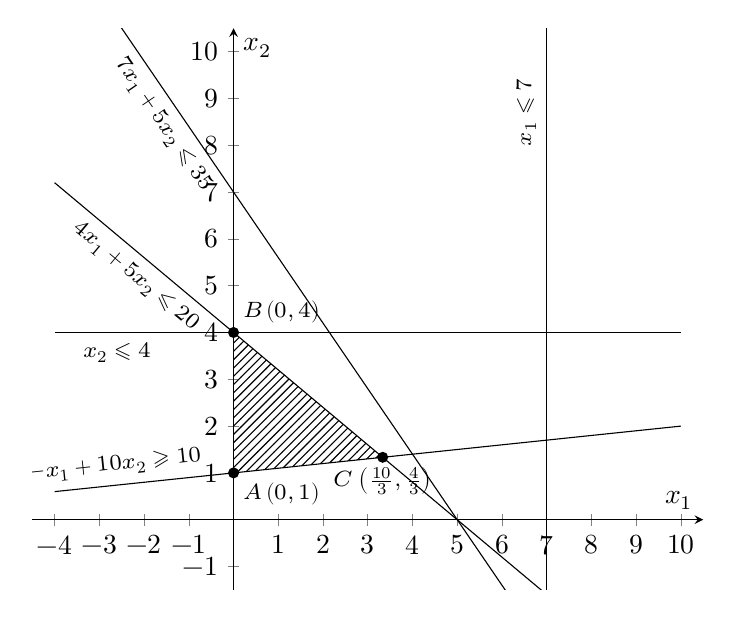
\begin{tikzpicture}[
        plot expl/.style = {sloped, font = {\footnotesize}},
      ]
        \begin{axis}[
          width=10\gridunitwidth,
          axis x line = middle,
          axis y line = middle,
          xmin = -4.5,
          xmax = 10.5,
          ymin = -1.5,
          ymax = 10.5,
          xtick distance = 1,
          ytick distance = 1,
          domain = -4:10,
          domain y = -1:10,
          xlabel = $x_1$,
          ylabel = $x_2$,
        ]
          \addplot [
            name path = 1,
          ] {
            (20 - 4*x) / 5
          }
            node [plot expl, below, pos=0.15] {$4 x_1 + 5 x_2 \leqslant 20$};

          \addplot [
            name path = 2,
          ] {
            (10 + x) / 10
          }
            node [plot expl, above, pos=0.10] {$-x_1 + 10 x_2 \geqslant 10$};
          ;

          \addplot [
            name path = 3,
          ] {
            (35 - 7*x) / 5
          }
            node [plot expl, below, pos=0.20] {$7 x_1 + 5 x_2 \leqslant 35$};
          ;

          % Draw x_1 = 7
          \draw ({axis cs:7,0}|-{rel axis cs:0,0}) -- ({axis cs:7,0}|-{rel axis cs:0,1})
            node [plot expl, above, pos=0.85] {$x_1 \leqslant 7$};

          % Draw x_2 = 4.
          \addplot [
            name path = 4,
          ] {
            4
          }
            node [plot expl, below, pos=0.10] {$x_2 \leqslant 4$};
          ;

          % Draw axes
          % OX
          \path [name path=xaxis] (axis cs: \pgfkeysvalueof{/pgfplots/xmin}, 0) -- (axis cs: \pgfkeysvalueof{/pgfplots/xmax}, 0);

          % OY
          \path [name path=yaxis] (axis cs: 0, \pgfkeysvalueof{/pgfplots/ymin}) -- (axis cs: 0, \pgfkeysvalueof{/pgfplots/ymax});

          % Draw solution space fill
          \addplot [gray, pattern=north east lines] fill between[
            of=1 and 2,
            soft clip = {
              domain = 0:3.35,
            }
          ];
          % Draw interseciton points
          \fill [name intersections = {of = 2 and yaxis}]
            (intersection-1) circle[radius = 2pt] node [below right] {\footnotesize$A\,(0, 1)$};

          \fill [name intersections = {of = 1 and 4}]
            (intersection-1) circle[radius = 2pt] node [above right] {\footnotesize$B\,(0, 4)$};

          \fill [name intersections = {of = 1 and 2}]
            (intersection-1) circle[radius = 2pt] node [below] {\footnotesize$C\,\left(\frac{10}{3}, \frac{4}{3}\right)$};
        \end{axis}
      \end{tikzpicture}
      \caption{Графік області можливих розв'язків}
      \label{fig:02-plot-explicit}
    \end{figure}

    Відомо, що~якщо задача лінійного програмування має~оптимальне рішення, то~воно співпадає з~однією (двома) вершинами многокутника обмежень. Отже, щоб~знайти оптимальне рішення, необхідно визначити вершину, при~якій значення функції найменше. Для~цього підставляємо значення координат у~цільову функцію і~знаходимо її~значення:
    \begin{IEEEeqnarray*}{rCl}
      L(A) &=& -4 \cdot 0 - 5 \cdot 1 = -5,\\
      L(B) &=& -4 \cdot 0 - 5 \cdot 4 = -20,\\
      L(C) &=& -4 \cdot \frac{10}{3} - 5 \cdot \frac{4}{3}
               = \frac{-40}{3} - \frac{20}{3}
               = \frac{-60}{3}
               = -20.
    \end{IEEEeqnarray*}
    Як~бачимо, цільова функція~$L$ набуває найменших значень у~точках~$B\,(0; 4)$ і~$C\,(10/3; 4/3)$, а~отже розв'язками задачі будуть такі пари значень керованих змінних: $x_{1} = 0, \, x_{2} = 4$ та~$x_{1} = 10/3, \, x_{2} = 4/3$.

  \section{Висновок}
    Виконуючи дану лабораторну роботу, ми~навчились використовувати графічний метод розв'язання задач лінійного програмування, а~також розробляти програмне забезпечення для~допомоги при~розв'язанні задачі лінійного програмування графічним методом.

  \appendix
  \section{Програма для~розв'язку поставленої задачі}
    \inputpython{../01-solution/y04s01-lab-01-02-solver.py}{Початковий код~програми для~побудови півплощин обмежень}{lst:01-solver-src}

\end{document}
